\documentclass[11pt,a4paper,english,twoside,openany]{book}

\usepackage{html}
\usepackage{hyperref}
\usepackage{doipubmed}
\usepackage{a4,graphicx,texdraw,amsmath,amssymb,natbib}
\usepackage{fancyhdr}
\usepackage{a4wide}
\usepackage{babel}
\usepackage{pdfpages}
\parskip 11pt

\newcommand{\beq}{\begin{equation}}
\newcommand{\eeq}{\end{equation}}
\newcommand{\beqn}{\begin{eqnarray}}
\newcommand{\eeqn}{\end{eqnarray}}


\begin{document}
\pagenumbering{arabic}

\pagestyle{empty}

\newcommand{\um}{$\mu$m}

\newcommand{\bx}{\mathbf{x}}
\newcommand{\bn}{\mathbf{n}}
\newcommand{\bnp}{\mathbf{n}'}

\title{SOCRATES User Guide\\
Suite Of Community RAdiative Transfer codes based on Edwards and Slingo}
\date{\today}

\author{James Manners, John M. Edwards, Peter Hill \& Jean-Claude Thelen\\
Met Office, FitzRoy Rd, Exeter EX1 3PB
\thanks{
 The contents of this document are Crown Copyright.
}}
\maketitle

\tableofcontents

\clearpage

\pagestyle{fancy}
\latex{
\fancyhf{}
\fancyhead[LE,RO]{\thepage}
\fancyhead[LO]{\nouppercase{\rightmark}}
\fancyhead[RE]{\nouppercase{\leftmark}}
}

\chapter{Overview}
The radiation code is a suite of scripts and programs designed to calculate
radiative fluxes or radiances. The core of the code is used with the 
Met Office's GCM for climate and NWP forecasts. In order to calculate 
the radiation fields, additional information is required covering the 
decomposition of the spectrum into bands: this information is held in a 
{\em spectral file} which can be generated by preprocessing software. It
is not, however, necessary to generate a new spectral file for every 
calculation of fluxes. Atmospheric profiles must be specified to the code
and these are presented in netCDF (or text CDL) format. Multiple atmospheric
columns can be treated simultaneously. Programs also exist to create and
manipulate netCDF and CDL files.

The preprocessing suite of programs contains software to specify the structure
of a spectral file, software to generate representations of gaseous absorption
using the correlated-$k$ distribution method, code to generate scattering data
for water droplets, ice crystals and aerosols, together with a number of other
utilities.

Within the core program, fluxes are calculated using two-stream methods, a
choice of approximations being available, whilst radiances are calculated
using spherical harmonics. Two-stream concepts are well-known, but it may be
worth saying a few words about the calculation of radiances. To give the very
briefest of descriptions, the angular variation of the radiance at a
point is decomposed into spherical harmonics:
\begin{equation}
I({\bf r}, {\bf n}) = \sum_{l=0}^\infty \sum_{m=-l}^l I_{lm} ({\bf r})
Y_l^m({\bf n})
\end{equation}
Thus, the coefficients $I_{l,m}$ depend only on the spatial position and
not on the direction of the ray (in practice only vertical variations are
allowed for). Here $\bf n$ is a vector of unit length, specifying the
direction of the ray, and may be described by the polar and azimuthal
angles $\theta$ and $\phi$. The functions $Y_l^m$ are orthogonal when
integrated over all angles:
\begin{equation}
\int_{\Omega} Y_l^m({\bf n}) Y_{l'}^{m'}({\bf n}) \, d\omega_{\bf n}
= \delta_{ll'}\delta_{mm'}
\end{equation}
Hence, if the $I_{lm}$ have been determined, the complete radiation field
at a point is specified. The radiance in a given direction may, in theory,
be calculated directly by evaluating the $Y_l^m$ in that
direction and summing the terms; although in practice we use the spherical
harmonic decomposition to define the scattered radiation and integrate
along a ray. Alternatively, if we require a flux,
say the upward flux integrated over the upward hemisphere $\Omega_+$, we
have
\begin{equation}
F^+= \int_{\Omega_+} I({\bf n}) ({\bf n}. {\hat {\bf z}}) \, d\omega_{\bf n}
= \sum_{l=0}^\infty \sum_{m=-l}^l I_{lm} \int_{\Omega_+} Y_l^m({\bf n})
({\bf n}. {\hat {\bf z}}) \, d\omega_{\bf n},
\end{equation}
so again a sum of the $I_{lm}$ results. The core of the program is thus
devoted to calculating these coefficients.




\chapter{Setup and Operation}
\section{Obtaining the code}
The master version of the radiation code is held under version control (FCM)
on the Met Office Science Repository Service (MOSRS) at
https://code.metoffice.gov.uk/trac/socrates/wiki. Development information and
instructions are available from this page. Releases are
made from specific revisions of the trunk and made available 
as a self-contained tar package.

To obtain the latest version of the code or to get an account on the MOSRS
please email the radiation code owner at the Met Office, currently
james.manners@metoffice.gov.uk. The code is freely available under a
BSD 3-clause licence.

Once extracted, instructions for compilation may be found within the
distribution's {\tt README} file.

The code is written in Fortran 95 and has primarily been tested with the Intel 
ifort and GNU gfortran compilers. Scripts are written in the korn or bash
shells and it is recommended that one of these is used as the command shell.
A local installation of the netCDF fortran libraries and modules is also
required if the netCDF functionality is to be used.

\section{Basic operation}

The running of the code can be split into three tasks. First, a spectral 
file must be produced or chosen from the standard configurations included;
next, the physical state of the atmosphere must be expressed in the form of
netCDF or text CDL files (as defined below), and finally 
the code can be run to calculate radiances, fluxes and heating rates. The
following chapters describe each of these tasks, but here
it will be useful to make some concise general remarks, beginning
with a description of the spectral file.

\section{The Spectral File}

Spectral information is read from the {\em spectral file} produced by the
preprocessor. Once a spectral file has been produced it may be stored for
future use. A number of standard versions are available in {\tt \$RAD\_DIR/data/spectra/}.

The spectral file is at the heart of the code, and whilst the details of 
its internal
structure need not be studied since this file is always written and read by
special subroutines, some idea of its contents will be helpful.
The file consists of a number of different blocks of data. Each block
begins with a line of the form

\begin{flushleft}
\hspace*{.5in}{\tt *BLOCK: TYPE =    $n_1$: SUBTYPE =     $n_2$: VERSION =     $n_3$}
\end{flushleft}

and ends with a line of the form

\begin{flushleft}
\hspace*{.5in}{\tt *END}
\end{flushleft}

The type number identifies the contents of the block; for example, type 10
is concerned with the properties of cloud droplets. The subtype is used to
give a more precise description of the contents of the block; for example
in the case or block 10 the subtype 1 indicates parametrized optical
properties whilst the subtype 2 indicates observational data. The version
number is included to allow the possibility of changing the format of
the blocks without losing backward compatibility with spectral files
produced using earlier versions of the code: one simply has different
input routines for each version. If the code is to be extended it is
possible to invent new types or subtypes of blocks and to provide routines
to read them. When the spectral file is read the main input subroutine
reads the title line as above and calls the correct routine to read the
rest of the block. Each block holds formatted data, and should therefore
be fairly readable by the user, should he wish to examine the data.

\section{The Structure of the Input Files}

In the radiation code the atmosphere is divided into a number of homogeneous
{\em layers} numbered downwards from 1 to $N$, these are bounded by {\em 
levels} numbered downwards from 0 to $N$. Input data is supplied as 
representative values in layers (equivalent to theta-levels in the UM).

The file format used is either CDL (ASCII files for use with l\_run\_cdl) 
or netCDF (binary files for use with l\_run\_cdf). Here, related fields 
are kept in separate files with a common
basename and a suffix referring to the contents of the file. For example,
{\tt xyz.t} will be profiles of atmospheric temperatures and {\tt xyz.ch4}
would be profiles of mass mixing ratios of methane. The suffixes known
to the code can be found in {\tt \$RAD\_BIN/input\_head\_pcf.f90}. Each file, 
whether netCDF or CDL (ASCII version of netCDF), contains a single variable 
named as the file suffix, with the dimensions given by longitude and latitude 
in the horizontal (although only a single point for CDL files) and pressure 
in the vertical. Extra variable attributes, such as longname (eg. Temperature), and units (eg. K) are also given.

To run the code we need to specify the pressure levels which bound the
layers and representative values of the fields within the layers,
given as values at the pressures at the mid-points of the
layers. Pressures are not read from a special file, but are taken from
the files of other fields, so care is necessary to ensure that all
profiles are consistent. In the case of infra-red radiation we need to
specify the temperatures at the edges of the layers: it is therefore
convenient always to specify the edges of the layers by having a file
of temperatures at the edges of layers, for which the suffix is {\tt
.tl}: this will contain $N+1$ rows of data if there are $N$ layers,
but all other files except those specifying surface (and top of
atmosphere) conditions will contain $N$ rows of data. The temperatures
at the mid-points of layers are  read from a file with the suffix {\tt
.t}. The surface pressure and temperature are set in files with the 
suffix {\tt .pstar} and {\tt .tstar} respectively. The surface albedo is 
given in {\tt .surf}. Top of atmosphere solar irradiance and solar zenith 
angle are given in {\tt .stoa} and {\tt .szen} respectively.

These files constitute the essential information necessary to run the code.
Depending on the options selected additional files will be required. If
gaseous absorption is included files of the mass mixing ratios of the gases
included in the spectral file will be required. If aerosols are to be
included appropriate mass mixing ratios will again be required. In the case
of clouds more information is required. A file with the suffix {\tt .clfr}
specifies the cloud fraction and files with the suffixes {\tt .lwm}, 
{\tt .re}, {\tt .iwm}, and {\tt .ire} give respectively the mass mixing
ratios of liquid water, the effective radius of cloud droplets, the mass
mixing ratio of ice crystals and the effective radius of ice crystals. Additional files will also be needed if radiances are to be calculated.


\section{Running the Code}

The code can be run in two ways. The simplest is to run the executable
interactively replying to the prompts. Fortran programs  {\tt l\_run\_cdl} or
{\tt l\_run\_cdf} will use this method. An alternative, which is often more
useful is to use a UNIX script (eg. {\tt Cl\_run\_cdl} or {\tt Cl\_run\_cdf}
respectively). These scripts process their input and write a temporary
file for the driver itself, run the driver and then remove the
temporary file. The options required to run these scripts are available 
from their {\tt man} pages:

\begin{verbatim}
man Cl_run_cdl
man Cl_run_cdf
\end{verbatim}

\subsection{Example data}

The directory {\tt examples} contains some example data which can be used to
test the code and provide models for other development.

The scripts {\tt quick\_tests} and {\tt slow\_tests} will run all the example
cases and compare the output with standard results from the ifort and gfortran
compilers used within the Met Office. These tests are expected to 'fail' with
minor differences if different compilers (or compiler versions) are used.


\chapter{Producing The Spectral File}

Before the main code can be run it is necessary to build a spectral file.
A number of programs are used in building the spectral file and detailed
descriptions are given in the next chapter. These programs can be run 
interactively or using UNIX scripts. This process is somewhat involved:
it may be most helpful to read the general discussion here first, then to
read carefully through the examples in the directory {\tt \$RAD\_DIR/examples}
making continual reference to the descriptions of programs found in the next
chapter.

The first step in this process is to design a spectrum, choosing the number
of spectral bands and the wavelengths which delimit them, the absorbers
which are active in each of the bands, the possible types of continua, and
the types of aerosols which are to be included. These data are entered into a 
skeletal spectral file using the program {\tt prep\_spec} (see the example
in section~\ref{sec:ex_spf}).

Having created the skeletal spectral file, the spectral data for 
different spectral
processes have to be generated. The procedure for each process is
self-contained and there is no need to consider processes in any particular
order, except that gaseous absorption and continuum absorption must
be considered together.

The correlated-$k$ method may be used to
generate data for line and continuum absorption. There is one program, 
{\tt corr\_k} which generates both the line and the continuum data, though
it must be run separately for each process. An example use of this
program can be found in {\tt \$RAD\_DIR/examples/corr\_k}.

Aerosols, cloud droplets and ice crystals all introduce scattering effects
for which 
parametrizations are required. The scattering properties of spherical
particles may be calculated from a Mie scattering code. For non-spherical
ice crystals, the use of predefined databases of propeties is preferred.
The scattering code for spherical particles is called {\tt scatter}. This
is a fairly general code which will generate single scattering properties at
a range of specified wavelngths, integrated over a distribution of sizes.
In the case of aerosols a parametrization of the effects of humidity due
to D.~L.~Roberts is available. The normal scattering algorithm is a Mie
scattering code based on that given by Bohren and Huffman. Data for ice
crystals may be generated from this code if they are modelled as spheres,
but in general databases of scattering propeties should be used.

These monochromatic single-scattering data, whether generated from the Mie
code or from the non-spherical code, must be averaged across bands and
possibly parametrized before being included in the spectral file. The
output from several runs of the scattering program may be concatenated to
make one large file for input to the program for averaging scattering data,
{\tt scatter\_average},
each sub-file being termed a block: this makes it possible, for example, to
feed in data generated with different effective radii for fitting. The 
program reads each block of data, averages the single scattering properties
across the bands of a spectral file and then fits a parametrization to these
averaged properties if required.

Once these files have been generated, the data must be inserted into the
spectral file: this is also done with the program {\tt prep\_spec} which allows
the user to append data to an existing spectral file, or to generate a new
file from an old one. On entry into the program the user is presented with
a menu of block numbers from which to select an action to make blocks of
that number. As well as providing gaseous or scattering data if they are 
required, the user can calculate the fraction of
the solar spectrum in each band, the Rayleigh scattering coefficients, the
surface properties, or a polynomial fit to the Planck function in each
band as required. There is no necessity to produce blocks of every type:
for example, if one did not wish to consider Rayleigh scattering in the
radiation code, there would be no need to calculate the scattering
coefficients. Of course, for solar calculations the fraction of the solar
spectrum in each band must be calculated, and for infra-red calculations a
fit to the Planck function is required. It is perfectly possible to add to
a spectral file at a later date, so one might have a spectral file including
gaseous and droplet data and now wish to add aerosol data: this file could
be used together with Mie data to run {\tt scatter\_average} to generate
averaged aerosol scattering properties, and these properties could then be
appended to the file. The minimum permissible content of a spectral file is
that which is produced when {\tt prep\_spec} is first run. We have previously
called this the skeletal spectral file, though this term should not be taken to
imply that it has any special and peculiar form.

Once the spectral file has been produced the radiation code can be run.
Note again that it is not necessary to generate a spectral file every time
the code is to be run. They may be kept in a library and used as appropriate.
Some standard files are kept in the directory {\tt \$RAD\_DATA/spectra}.

\section{An Example}
\label{sec:ex_spf}

The following is a copy of the script file generated during the production
of an example spectral file: this is purely illustrative and choices of gases
and bands have not been made on scientific grounds.

The skeletal spectral file must be prepared first. Here we have selected 
two bands from 4.4-- 4.5 \um\ and from 4.6 to 4.7 \um, but we wish to excise
the region from 4.61 -- 4.62 \um\ from the second band for separate treatment.
What this means in effect is that the two regions 4.60 -- 4.61 \um\ and
4.62 -- 4.70 \um\ will be treated as one band. (This option is only really
relevant in a GCM, where, for example, we might have one band covering 
the whole atmospheric window from 8 -- 12 \um, but would wish to exclude 
the 9.6 \um\ band of ozone for separate treatment. By doing this we can use only
one set of $k$-terms for both parts of the band, allowing faster execution.)
The first and second bands include absorption by water vapour, the second
also including absorption by carbon dioxide and nitrous oxide, but only
carbon dioxide is considered in the excluded band. The self and 
foreign-broadened continua of water vapour are also included, together with 
two aerosols.

{\small
\begin{verbatim}
$ prep_spec
Enter the name of the spectral file.
sp_ex
A new spectral file will be created.

Enter number of spectral bands.

3

Enter number of absorbing gases.

3

Enter the physical types of absorber.
Enter the identifier for gas      1
1
Enter the identifier for gas      2
4
Enter the identifier for gas      3
2

Enter number of aerosols.

2

Enter the physical types of aerosol.
Enter the identifier for aerosol      1
3
Enter the identifier for aerosol      2
7

For each band in turn specify the limits of the bands in 
metres, inverse centimetres or microns.

type "m" for metres, "c" for inverse centimetres, or "u" for microns.
u
Enter limits for band     1
4.4 4.5
Enter limits for band     2
4.6 4.7
Enter limits for band     2
4.61 4.62
All bands specified.




For each band specify the type numbers of the absorbers
active in that band.
To continue input on the next line terminate the line with an &.
enter '0' if there is no gaseous absorption in the band.

identifiers of absorbers in band        1
1
identifiers of absorbers in band        2
4 1 2
identifiers of absorbers in band        3
2


For each band, specify the types of the continuum absorbers 
active in that band.
To continue input on the next line terminate the line with an &.


Enter "0" if there is no continuum absorption in the band.

type numbers of continua in band      1
1
type numbers of continua in band      2
1 2
type numbers of continua in band      3
1


Do you wish to exclude regions from particular bands? (y/n)
y
For each band enter the list of bands to be excluded therefrom.
To continue input on the next line terminate the line with an &.

Enter '0' if no bands are to be excluded.

bands excluded from band      1
0
bands excluded from band      2
3
bands excluded from band      3
0

Select from the following types of data:
      2.   Block 2: Solar spectrum in each band.
      3.   Block 3: Rayleigh scattering in each band.
      5.   Block 5: k-terms and p, T scaling data.
      6.   Block 6: Thermal source function in each band.
      9.   Block 9: Continuum extinction and scaling data.
      10.  Block 10: Droplet parameters in each band.
      11.  Block 11: Aerosol parameters in each band.
      12.  Block 12: Ice crystal parameters in each band.
      -1.  To write spectral file and exit.
      -2.  To quit without writing spectral file.


-1
\end{verbatim}
}

Gaseous transmissions should then be generated from spectroscopic data
using the {\tt corr\_k} program.

\section{An Example Including an instrumental response function}
To simulate satellite radiances, or observational data more generally,
account must be taken of the instrumental response function. This involves
weighting data at various stages of the process of generating data.
This example is based on setting up a file for the Seviri 3.9 micron channel.

This filter response for this channel is zero outside the range 3.05--4.79
microns. This range include the 4.3 micron band of CO${}_2$ and a little
absorption by water vapour. CO2 is therefore the dominant absorber in the
channel. We first define the skeleton of the spectral file.

{\small
\begin{verbatim}
$ prep_spec
Enter the name of the spectral file.
sp_sw_sv39
A new spectral file will be created.

Enter number of spectral bands.
1

Enter number of absorbing gases.
2

Enter the physical types of absorber.
Enter the identifier for gas      1
2
Enter the identifier for gas      2
1

Enter number of aerosols.
2

Enter the physical types of aerosol.
Enter the identifier for aerosol      1
2
Enter the identifier for aerosol      2
10

For each band in turn specify the limits of the bands in 
metres, inverse centimetres or microns.

type "m" for metres, "c" for inverse centimetres, or "u" for microns.
u
Enter limits for band     1
3.05 4.79
All bands specified.


For each band specify the type numbers of the absorbers
active in that band.
To continue input on the next line terminate the line with an &.
enter '0' if there is no gaseous absorption in the band.

identifiers of absorbers in band        1
2 1


For each band, specify the types of the continuum absorbers 
active in that band.
To continue input on the next line terminate the line with an &.


Enter "0" if there is no continuum absorption in the band.

type numbers of continua in band      1
1


Do you wish to exclude regions from particular bands? (y/n)
n
\end{verbatim}
}

The spectral file now looks as follows:

{\small
\begin{verbatim}
*BLOCK: TYPE =    0: SUBTYPE =    0: VERSION =    2
Summary of spectral data.
Number of spectral bands =     1
Total number of gaseous absorbers =     2
Total number of aerosols =     2
List of indexing numbers and absorbers.
Index       Absorber(identifier and name)
    1           2       Carbon Dioxide      
    2           1       Water Vapour        
List of indexing numbers of aerosols.
Index       Aerosol(type number and name)
    1           2       Dust-like           
    2          10       Accum. Sulphate     
*END
*BLOCK: TYPE =    1: SUBTYPE =    0: VERSION =    0
Specification of spectral intervals
Limits of spectral intervals (wavelengths in m.)
Band        Lower limit         Upper limit
    1        3.050000000E-06     4.790000000E-06
*END
*BLOCK: TYPE =    4: SUBTYPE =    0: VERSION =    0
Gaseous absorbers in each interval
(The number is the indexing number of the species as set out
 in the summary block 0.)
A zero indicates that there in no gaseous absorption in the interval.
Band        Number of active absorbers followed by indexing numbers
    1           2
         1    2
*END
*BLOCK: TYPE =    8: SUBTYPE =    0: VERSION =    0
Continuum absorbers in each interval
(The number is the indexing number of each type as set out
 in the module rad_pcf.)
A zero indicates that there is no continuum absorption in the interval.
Band         Number of active continua followed by indexing numbers
    1           1
         1
Indexing numbers of gases for continua:
     Index of water =     2
*END
\end{verbatim}
}

We next need to generate a fit for the gaseous data in this file using 
correlated-k methods. This uses the program {\tt corr\_k} (Note: The
environment variable \$RAD\_DATA should be expanded and the HITRAN file
02\_HIT96.par will be required in the working directory. Here we will
show the interactive form of the program. Alternatively the {\tt Ccorr\_k}
script could be used.):

{\small
\begin{verbatim}
$ corr_k

Give the name of the LbL absorption coefficient file.
co2_lbl.nc

Will a HITRAN database be provided? Type:
  L for line database (.par)
  X for cross-section database (.xsc)
  N for none.
l

Give the name of the HITRAN .par database.
02_hit12.par

Enter location of parsum.dat.
$RAD_DATA/gases/parsum.dat

Enter the name of the spectral file.
sp_sw_sv39

Is an instrumental response required? (Y/N)
y

Give the instrumental response.
$RAD_DATA/channels/seviri_ir39
Are line absorption data to be generated? (Y/N)
y
Are foreign continuum data to be generated? (Y/N)
n
Are self_broadened continuum data to be generated? (Y/N)
n
Enter the identifier for the gas to be considered.
2

Enter first and last bands to be considered.
1 1

Setting of pressures and temperatures:

Enter "f" to read from a file or "i" to set values interactively.
i
Specify pressure and corresponding temperatures (*END to finish)
6.00e3 190. 210. 230.
Specify pressure and corresponding temperatures (*END to finish)
1.25e4 190. 210. 230.
Specify pressure and corresponding temperatures (*END to finish)
2.50e4 200. 225. 250.
Specify pressure and corresponding temperatures (*END to finish)
5.00e4 225. 250. 275.
Specify pressure and corresponding temperatures (*END to finish)
1.00e5 250. 275. 300.
Specify pressure and corresponding temperatures (*END to finish)
*END
Are scaling functions/lookup tables required? (Y/N)
y

Enter the type of scaling function.
2

Are the reference conditions to be set interactively or from a file? (I/F)
i
Enter reference pressure and temperature in band     1
2.50e4 225.0

Enter the line-cutoff in m-1
2500.0

Enter the frequency increment for integration in m-1
1.0

Enter the type of c-k fit required.

1

Enter the tolerance for the fit.

1.0e-2

Enter the maximum pathlength for the absorber.

10.0

Select the method of weighting the transmittances.
    1. Planckian weighting at transmission temperature.
    2. Differential planckian weighting at transmission temperature.
    3. TOA solar spectral weighting.
    4. Uniform weighting.
Enter required number.

3

Enter the name of the file containing the solar irradiance data.
$RAD_DATA/solar/kurucz_95_reduced

Give the name of the output file.
svswfit_co2

Give the name of the monitoring file.
svswfit_mon_co2
===============================
corr_k : Execution starts 
 at 17:04:05 on 04/04/2014
Band   1 limits adjusted to:  208768.000  327869.000 m-1
===============================
Processing band     1
Gas required:    CO2
Band limits:  2062.680000   3303.690000
Opened HITRAN data file 
Number of HITRAN lines in band: 116100
Wavenumbers of min and max lines are:  1938.637060   3427.784093
Calculation of absorption coefficients at  6.000E+03 Pa and  1.900E+02 K
Calculation of absorption coefficients at  6.000E+03 Pa and  2.100E+02 K
Calculation of absorption coefficients at  6.000E+03 Pa and  2.300E+02 K
Calculation of absorption coefficients at  1.250E+04 Pa and  1.900E+02 K
Calculation of absorption coefficients at  1.250E+04 Pa and  2.100E+02 K
Calculation of absorption coefficients at  1.250E+04 Pa and  2.300E+02 K
Calculation of absorption coefficients at  2.500E+04 Pa and  2.000E+02 K
Calculation of absorption coefficients at  2.500E+04 Pa and  2.250E+02 K
Calculation of absorption coefficients at  2.500E+04 Pa and  2.500E+02 K
Calculation of absorption coefficients at  5.000E+04 Pa and  2.250E+02 K
Calculation of absorption coefficients at  5.000E+04 Pa and  2.500E+02 K
Calculation of absorption coefficients at  5.000E+04 Pa and  2.750E+02 K
Calculation of absorption coefficients at  1.000E+05 Pa and  2.500E+02 K
Calculation of absorption coefficients at  1.000E+05 Pa and  2.750E+02 K
Calculation of absorption coefficients at  1.000E+05 Pa and  3.000E+02 K
 Number of k-terms in band:            6
===============================
corr_k : Execution ends   
 at 17:08:39 on 04/04/2014
===============================
\end{verbatim}
}

The generated fit can then be added to the spectral file using
{\tt prep\_spec}:

{\small
\begin{verbatim}
$ prep_spec
Enter the name of the spectral file.
sp_sw_sv39
Type "a" to append data to the existing file;
  or "n" to create a new file.
a

Select from the following types of data:
      2.   Block 2: Solar spectrum in each band.
      3.   Block 3: Rayleigh scattering in each band.
      5.   Block 5: k-terms and p, T scaling data.
      6.   Block 6: Thermal source function in each band.
      9.   Block 9: Continuum extinction and scaling data.
      10.  Block 10: Droplet parameters in each band.
      11.  Block 11: Aerosol parameters in each band.
      12.  Block 12: Ice crystal parameters in each band.
      -1.  To write spectral file and exit.
      -2.  To quit without writing spectral file.


5

enter the name of the file of esft data.
svswfit_co2
\end{verbatim}
}

This will add the following block to the spectral file for the CO2
absorption coefficients (6 k-terms):

{\small
\begin{verbatim}
*BLOCK: TYPE =    5: SUBTYPE =    0: version =    1
Exponential sum fiting coefficients: (exponents: m2/kg)
Band        Gas, Number of k-terms, Scaling type and scaling function,
             followed by reference pressure and temperature,
                   k-terms, weights and scaling parameters.
    1           1           6           2           2
       2.500000000E+04       2.250000000E+02
    4.820386294E-04    9.356713378E-01    1.989931390E-01    1.923337296E+00
                                         -1.309827391E+00
    3.246306915E-01    2.993051740E-02    8.797685008E-01    2.311229496E+00
                                         -1.265889618E+00
    1.097340512E+01    1.367939377E-02    8.105283591E-01    1.268958997E+00
                                         -1.664535414E+00
    1.110700060E+02    1.708563272E-02    8.029082834E-01    3.824743186E-03
                                         -1.006268013E+00
    2.306389704E+03    2.948210815E-03    4.808108016E-01   -1.509617263E-01
                                         -2.860907846E+00
    5.015212272E+04    6.849075190E-04   -2.813477713E-01   -3.104128796E-01
                                         -3.377901661E+00
    1           2           1           0           0
       1.236858101-312       1.236858101-312
    0.000000000E+00    1.000000000E+00
*END
\end{verbatim}
}

\section{Generating Scattering Data}
The scattering properties of particles can be calculated directly
using electromagnetic theory; but even for a shape so simple as
a sphere this would be prohibitively expensive in a radiation
code. Therefore, scattering propeties are calculated outside the
radiation code and represented in a parametrized form within it.

For aerosols, water droplets and ice crystals, the procedure is
generically similar, although there are subtle nuances. Water
droplets are spherical and aerosols are at the present time 
treated as spherical. Over recent years it has become possible
to treat non-spherical ice crystals and this makes the treatment
of ice more dissimilar from the other two types of particle.

In any region of the atmosphere there will be a mixture of particles
of different sizes, so a size ditribution must be considered. For
water droplets and aerosols, simple analytic distributions such
as the log-normal or modified gamma distributions are often assumed.
Size distributions for ice crystals are much less regular and often
bimodal; we are tending now to use observational size distributions
to generate scattering data for ice crystals.
 
Having assumed a size distribution, it is necessary to calculate the
individual scattering properties of particles of a given size before
avaeraging across the size distribution. In the case of aerosols and
droplets, Mie scattering calculations are done, but for non-spherical
ice crystals, it would be too complicated to do these calculations
all at once and an external database is used. To do Mie calculations,
a file of refractive indices is required.

The generic procedure, then, is that single scattering propeties are
generated at a number of frequencies, averaged over a size distribution
using the program {\tt scatter}. These must then be averaged over the
bands of the spectral file, weighting with a solar spectrum or a
Planckian function (and including an instrumental response if necessary).
In the case of droplets and ice crystals we need to consider a range
of size distributions and generate a fit in terms of particle size.
This is done using the program {\tt scatter\_average}.

We shall now consider aerosols, droplets and ice crystals in turn. The
detailed description of the programs should also be consulted.

\subsection{Generating Scattering data for aerosols}
The script below is an example of the generation of aerosol data.
Having generated the skeletal spectral file, we run {\tt scatter} to
generate monochromoatic single scattering data. The wavelengths are
in the file {\tt \$RAD\_DATA/aerosol/wl\_aerosol} and the refractive
indices for several aerosols are also stored under {\tt \$RAD\_DATA/aerosol}.
{\tt -C} introduces the
component (or type of aerosol) and {\tt -l} enforces linear interpolation
of the refractive indices in frequency. A log-normal distribution is 
used ({\tt -g}), with a total number density of $1\times 10^8$. 21
moments of the phase function are generated. For hygroscopic aerosols,
we also need to consider the growth with humidity, as shown in the
second invocation. Aerosol data are averaged across spectral bands
using {\tt Cscatter\_average} as shown. Note the option to average
a smaller number of moments of the phase function than were generated
when running {\tt scatter}: this allows the expensive scattering 
program to be run just once and perhaps to be used to generate different
spectral files.

{\small
\begin{verbatim}
#! /bin/ksh
#
# Example script showing the generation of aerosol scattering data.
#
# 0.) Set the path for the radiation code
#
. $RAD_DIR/set_rad_env
#
# 1.) Make spectrum with prep_spectrum
#     See previous example to create sp_sw_sv39.
#
# 2.) Generate aerosol scattering data.
#
Cscatter -w $RAD_DATA/aerosol/wl_aerosol \
  -r $RAD_DATA/aerosol/refract_dust -C 2 -l \
  -g 1.0 5.0e-7 1.05 -n 1.e8 -o fl_dust_sct -P 21 -t 1 -M
#
# With humidity dependence
#
Cscatter -w $RAD_DATA/aerosol/wl_aerosol \
  -r $RAD_DATA/aerosol/refract_ammoniumsulphate -C 10 -l \
  -g 1.0 5.0e-7 1.05 -n 1.e8 -o fl_aero_sct -P 21 -t 1 -M \
  -h $RAD_DATA/cloud/refract_water \
     $RAD_DATA/aerosol/humidities
#
# 3.) Average across the bands of the spectral file
#
Cscatter_average -s sp_sw_sv39 -P 19 \
  -S $RAD_DATA/solar/kurucz_95_reduced -w  \
  -i $RAD_DATA/channels/seviri_ir39 \
  -a fl_dust_avv fl_dust_sct
Cscatter_average -s sp_sw_sv39 -P 19 \
  -S $RAD_DATA/solar/kurucz_95_reduced -w  \
  -i $RAD_DATA/channels/seviri_ir39 \
  -a fl_aero_avv fl_aero_sct
\end{verbatim}
}

\subsection{Generating Scattering data for water droplets}
Generating data for droplets is in many ways like generating data
for aerosols, but using a single size distribution (one inovcation
of {\tt scatter}) yields only one effective particle size. In this
case, however, we require a range of sizes to do a fit in the 
effective radius. {\tt scatter} must therefore be run several
times and the results concatenated together for input to 
{\tt scatter\_average} as shown.

{\small
\begin{verbatim}
#! /bin/ksh
#
# Example scattering script for droplets
#
. $RAD_DIR/set_rad_env
#
# 1.) Make spectrum with prep_spectrum
#     See previous example to create sp_sw_sv39.
#
# 2.) Generate scttering data for droplets. We need to do
#     this for a range of droplet distributions. For this
#     example we have ludicrously small droplets.
#
Cscatter -w $RAD_DATA/cloud/wl_cloud -r $RAD_DATA/cloud/refract_water \
  -g 1.0 5.0e-7 1.02 -n 1.e8 -o gl_drop_sct_0 -P 21 -t 2 -M -U 1 -l
Cscatter -w $RAD_DATA/cloud/wl_cloud -r $RAD_DATA/cloud/refract_water \
  -g 1.0 6.0e-7 1.09 -n 1.e8 -o gl_drop_sct_1 -P 21 -t 2 -M -U 1 -l
Cscatter -w $RAD_DATA/cloud/wl_cloud -r $RAD_DATA/cloud/refract_water \
  -g 1.0 7.0e-7 1.08 -n 1.e8 -o gl_drop_sct_2 -P 21 -t 2 -M -U 1 -l
Cscatter -w $RAD_DATA/cloud/wl_cloud -r $RAD_DATA/cloud/refract_water \
  -g 1.0 8.0e-7 1.07 -n 1.e8 -o gl_drop_sct_3 -P 21 -t 2 -M -U 1 -l
Cscatter -w $RAD_DATA/cloud/wl_cloud -r $RAD_DATA/cloud/refract_water \
  -g 1.0 9.0e-7 1.06 -n 1.e8 -o gl_drop_sct_4 -P 21 -t 2 -M -U 1 -l
Cscatter -w $RAD_DATA/cloud/wl_cloud -r $RAD_DATA/cloud/refract_water \
  -g 1.0 1.0e-6 1.05 -n 1.e8 -o gl_drop_sct_5 -P 21 -t 2 -M -U 1 -l
#
# Combine all scattering data into one file.
#
cat gl_drop_sct_? > gl_drop_all
#
# 3.) Average across the bands of the spectral file and fit. 
#
Cscatter_average -s sp_sw_sv39 -P 19 \
  -S $RAD_DATA/solar/kurucz_95_reduced -t  \
  -i $RAD_DATA/channels/seviri_ir39 \
  -a gl_drop_avv -f 6 gl_drop_fit gl_drop_mon 1.e3 gl_drop_all
\end{verbatim}
}
\subsection{Generating Scattering data for ice crystals}
Because of their irregular shapes, calculating the scattering properties
of ice crystals is considerably more complicated than calculating the
scattering propeties of a water droplet. Whilst it is possible to
generate data using a Mie scattering code treating ice crystals as
spheres, this approach is largely out of date. The preferred approach
now is to use a database of scattering properties prepared using
appropriate off-line algorithms. 
Databases are too varied to be considered as an integral part of the 
radiation code and some coding to use a particular new database should
be expected.

\section{Generating solar spectral variability data}
\label{sec_spectral_var}

For some applications (such as long climate runs of the Met Office Unified Model) it is necessary to account for changes in the solar spectrum and total solar irradiance with time. The proportion of the solar spectrum in each band is provided in block 2 of the shortwave spectral file. Optical properties given in other blocks will also generally be weighted by the underlying solar spectrum so should ideally also change as the solar spectrum changes with time. The most important of these are the spectral weightings given to gaseous absorption coefficients in block 5 and the spectrally weighted averages of the Rayleigh scattering coefficients in block 3. To a certain degree changes in these coefficients with time can now be specified using a look-up table in block 17 of the spectral file.

Block 17 specifies sub-band wavelength ranges for which solar spectral variations may be specified in an accompanying {\tt spectral\_var} file. Sub-bands are generally equivalent to the full bands except for particular cases where the weights for the k-terms of the major gas in the band actually represent a particular wavelength interval within the band. This is best illustrated with reference to the GA7 shortwave spectral file which contains sub-bands for ozone absorption in the ultra-violet. The script which generated these ozone k-terms can be seen in {\tt \$RAD\_DIR/examples/sp\_sw\_jm/mk\_sp\_sw\_6\_jm2}. A 12-band skeleton spectral file has been used where the first 6 bands correspond to band 1 of the GA7 spectral file, and bands 7-8 correspond to band 2 of the GA7 spectral file. A single ozone k-term has been generated for each of the first 8 bands of the 12-band skeleton spectral file. These have then been converted to 6 k-terms for band 1, and 2 k-terms for band 2 of the GA7 file by using the normalised solar spectrum fraction as the k-term weights. Here, we can now specify the original 12 spectral intervals as sub-bands in block 17. With solar spectral variations supplied for each of these sub-bands it is then possible for the code to vary the ozone k-term weights appropriately for the solar spectrum. 

Here we run through the example given in {\tt \$RAD\_DIR/examples/spectral\_var} for the creation of a look-up table of solar spectral variability data. The raw spectral variability data files recommended for CMIP5 are first downloaded:

{\small
\begin{verbatim}
wget http://solarisheppa.geomar.de/solarisheppa/sites/default/files/
              ...                     data/CMIP5/spectra_1610_2000a_21Jan09.txt.gz
              ...                     data/CMIP5/spectra_1882_2000m_17Dec08.txt.gz
              ...                     data/CMIP5/spectra_2000_2008m_6May09.txt.gz
gunzip *.gz
\end{verbatim}
}

\noindent The format of these files is understood by the {\tt prep\_spec} program which is then run to create block 17 of the spectral file:

{\small
\begin{verbatim}
$ prep_spec
Enter the name of the spectral file.
sp_sw_ga7
Type "a" to append data to the existing file;
  or "n" to create a new file.
a

Select from the following types of data:
      2.   Block 2: Solar spectrum in each band.
      3.   Block 3: Rayleigh scattering in each band.
      5.   Block 5: k-terms and p, T scaling data.
      6.   Block 6: Thermal source function in each band.
      9.   Block 9: Continuum extinction and scaling data.
      10.  Block 10: Droplet parameters in each band.
      11.  Block 11: Aerosol parameters in each band.
      12.  Block 12: Ice crystal parameters in each band.
      17.  Block 17: Spectral variability data in sub-bands.
      -1.  To write spectral file and exit.
      -2.  To quit without writing spectral file.


17
\end{verbatim}
}

\noindent For this example block 17 does not yet exist so we need to specify which of the bands can be further sub-divided into sub-bands (if the block does exist then this part is skipped and we can choose to add spectral variability data directly):

{\small
\begin{verbatim}
Enter band to be sub-divided (0 to finish): 
1
There are     6 major gas k-terms in this band.
Do you want to divide equally in wavelength (E),
or provide band limits (L) for each k-term?
e

Enter band to be sub-divided (0 to finish): 
2
There are     2 major gas k-terms in this band.
Do you want to divide equally in wavelength (E),
or provide band limits (L) for each k-term?
l
Enter band limits (metres): 
320.e-9 400.e-9
400.e-9 505.e-9

Enter band to be sub-divided (0 to finish): 
0
\end{verbatim}
}

\noindent Now we deal with the treatment of Rayleigh scattering coefficients for the varying solar spectrum. We may choose to specify time varying Rayleigh coefficients for only some of the sub-bands, so it is necessary for block 17 to contain default values for each sub-band calculated using the original mean solar spectrum used for blocks 2 and 3. Here we specify that only the first 8 sub-bands will have Rayleigh coefficients in the time-varying look-up table (generally variations are only important for the shorter wavelengths).

{\small
\begin{verbatim}
A mean solar spectrum is needed for the mean
Rayleigh coefficients per sub-band:

Enter the name of the file containing the solar irradiance data.
../../data/solar/lean_12

Is the atmosphere composed of air or H2-He gas (A/H)?
a
How many sub-bands will require a varying Rayleigh coefficient:
8
\end{verbatim}
}

\noindent We could have specified 0 here so that no Rayleigh coefficients would be given in the look-up table at all. In that case the default sub-band values would be used, but combined with the appropriate sub-band solar fraction at each time. In the case of band 1 this would still have provided the majority of the variation as the first 6 sub-band values would be appropriately weighted as the spectrum varied.

This completes the creation of block 17 in the main spectral file. The program continues with the addition of spectral variability data for each time. If block 17 had already existed in the spectral file {\tt prep\_spec} would jump directly to this point to allow times to be added to the spectral variability data.

{\small
\begin{verbatim}
Number of times / dates to add to spectral data
272
Enter format of data file:
5
Enter location of data file:
spectra_1610_2000a_21Jan09.txt

Number of times / dates to add to spectral data
1416
Enter format of data file:
5
Enter location of data file:
spectra_1882_2000m_17Dec08.txt

Number of times / dates to add to spectral data
108
Enter format of data file:
5
Enter location of data file:
spectra_2000_2008m_6May09.txt

Number of times / dates to add to spectral data
0
\end{verbatim}
}

\noindent Finally, we specify how many of the last times given should be repeated into the future. Here we are using monthly data so by specifying 144 we will have the final 12 years (1997-2008 inclusive: cycle 23) periodically repeated for as long as the model runs.

{\small
\begin{verbatim}
How many of the final times / dates should be 
periodically repeated into the future:
144

Select from the following types of data:
      2.   Block 2: Solar spectrum in each band.
      3.   Block 3: Rayleigh scattering in each band.
      5.   Block 5: k-terms and p, T scaling data.
      6.   Block 6: Thermal source function in each band.
      9.   Block 9: Continuum extinction and scaling data.
      10.  Block 10: Droplet parameters in each band.
      11.  Block 11: Aerosol parameters in each band.
      12.  Block 12: Ice crystal parameters in each band.
      17.  Block 17: Spectral variability data in sub-bands.
      -1.  To write spectral file and exit.
      -2.  To quit without writing spectral file.


-1
\end{verbatim}
}

\noindent The spectral file produced will now have a block 17 that looks like this:

{\small
\begin{verbatim}
*BLOCK: TYPE =   17: SUBTYPE =    0: VERSION =    0
Specification of sub-bands for spectral variability data.
Wavelength limits (m) and Rayleigh coefficients at STP (m2/kg).
Number of spectral sub-bands = 12
Sub-band Band  k-term     Lower limit         Upper limit       Rayleigh coeff
    1      1      1     2.000000000E-07     2.200000000E-07     5.411639620E-04
    2      1      2     2.200000000E-07     2.400000000E-07     3.808912673E-04
    3      1      3     2.400000000E-07     2.600000000E-07     2.532462086E-04
    4      1      4     2.600000000E-07     2.800000000E-07     1.841386263E-04
    5      1      5     2.800000000E-07     3.000000000E-07     1.319010864E-04
    6      1      6     3.000000000E-07     3.200000000E-07     1.006372358E-04
    7      2      1     3.200000000E-07     4.000000000E-07     5.509622529E-05
    8      2      2     4.000000000E-07     5.050000000E-07     2.147544832E-05
    9      3      0     5.050000000E-07     6.900000000E-07     7.463127997E-06
   10      4      0     6.900000000E-07     1.190000000E-06     1.639144948E-06
   11      5      0     1.190000000E-06     2.380000000E-06     1.788411198E-07
   12      6      0     2.380000000E-06     1.000000000E-05     1.082347954E-08
*END
\end{verbatim}
}

\noindent The mapping from sub-band to true band is provided along with the particular major gas k-term the sub-band applies to. A zero in the k-term column indicates that the sub-band represents the entire true band. 

An additional file called {\tt sp\_sw\_ga7\_var} has also been produced with data in this format (initially annual variation with monthly data beginning from 1882):

{\small
\begin{verbatim}
Number of times in look-up table = 1796
Number of times for periodic repetition = 144
Number of Rayleigh coefficients given = 8
Year  Month  Day(of month)  Seconds(since midnight)  TSI(Wm-2 at 1 AU)
Fraction of solar flux in each sub-band.
Rayleigh coefficient in the first 8 sub-bands.
*BEGIN: spectral variability data
  1610     1     1     0     1.360767554E+03
 4.190367994E-04 6.914841802E-04 9.624859423E-04 2.832880852E-03 5.910684856E-03
 9.261289946E-03 5.963858761E-02 1.460351240E-01 2.322715146E-01 3.224999155E-01
 1.813335685E-01 3.814342695E-02
 5.408985990E-04 3.808910747E-04 2.531982401E-04 1.841411970E-04 1.318903129E-04
 1.006353079E-04 5.509924875E-05 2.147515176E-05
  1611     1     1     0     1.360750657E+03
 4.187034033E-04 6.911699475E-04 9.621671540E-04 2.832480888E-03 5.910305453E-03
 9.260996582E-03 5.963753417E-02 1.460347926E-01 2.322714839E-01 3.225014149E-01
 1.813353418E-01 3.814360881E-02
 5.408868352E-04 3.808910741E-04 2.531961229E-04 1.841412817E-04 1.318898392E-04
 1.006352283E-04 5.509938863E-05 2.147514454E-05
\end{verbatim}
}

\noindent When this data is used in the Met Office Unified Model the values at the last date / time before the current timestep will be taken without interpolation.


\chapter{Preprocessing programs}
The following programs can be used to generate data for the spectral file. The names of the interactive Fortran programs are listed. Scripts are also available for most programs (beginning with ``C'') to call the respective Fortran routines after reading command line options. Man pages for these scripts (where available) are provided at the end of the chapter.

\begin{description}

\item[{\tt corr\_k}]
This program calculates correlated-$k$ coefficients for prescribed
spectral bands using data from HITRAN .par (line absorption) files,
.xsc (cross-section) files or .cia (collision-induced absorption)
files. It will also calculate water vapour continuum absorption
across the band.

A man page for Ccorr\_k is provided.

\item[{\tt scatter\_90}]
This program calculates the monochromatic single scattering
properties of spherical particles averaged over a size distribution
at a range of specified wavelengths.

A file of wavelengths for the calculation and a file of
refractive indices are read in. A distribution and a
scattering algorithm are supplied. The program calculates
single scattering properties at each of the wavelengths given.

A man page for Cscatter is provided.

\item[{\tt scatter\_average\_90}]
This program reads a file of monochromatic single-scattering
data and averages them across the bands specified in a spectral
file. The averaged values may be written to
a file or fitted using a recognized parametrization.

A man page for Cscatter\_average is provided.

\item[{\tt prep\_spec}]
This program is used to interactively construct a spectral file,
either entirely from scratch or based on an existing file.
For a new file the user is asked to supply the limits on the
spectral bands and the gases and aerosols present. Alternatively,
a spectral file is read in. The user then selects a block of data
to add to the file:

Block 2: Solar spectrum in each band.

Block 3: Rayleigh scattering in each band.

Block 5: k-terms and p, T scaling data.

Block 6: Thermal source function in each band.

Block 9: Continuum extinction and scaling data.

Block 10: Droplet parameters in each band.

Block 11: Aerosol parameters in each band.

Block 12: Ice crystal parameters in each band.

Block 17: Spectral variability data in sub-bands.

Block 19: Continuum k-terms and T scaling data.

Blocks 5, 9 \& 19 require output from the {\tt corr\_k} program.
Blocks 10, 11 \& 12 use output from {\tt scatter\_average}. Block 2 
requires a solar spectrum (examples are in \$RAD\_DATA/solar/).
Block 17 requires high-resolution solar spectral variability data files.
Formats accepted are currently:

CMIP5 (available from http://solarisheppa.geomar.de/cmip5).

CMIP6 (available from http://solarisheppa.geomar.de/cmip6)

The other blocks are compiled within the prep\_spec routine.

This routine is only available in interactive form. There are no command
line options and currently no man page.

\end{description}

Man pages follow formatted using {\tt man -t}.

\includepdf[pages=-]{Ccorr_k.pdf}
\includepdf[pages=-]{Cscatter.pdf}
\includepdf[pages=-]{Cscatter_average.pdf}


\chapter{Producing the Input Files}
The following programs can be used to generate input data for the radiance and two-stream code. As in the previous chapter the names of the Fortran programs are listed. Man pages for the corresponding scripts (where available) are then provided. 

\begin{description}

\item[{\tt raw\_input}]
: This is a possibly convenient way of making CDL-files specifying the
atmospheric state. We first need an input file. The input file
contains a number of {\sl profiles} beginning and ending with the
directives {\tt *PROFILE} and {\tt *END} (see {\tt examples/prsc/input}).
After the directive {\tt *PROFILE},
a line listing the variables to be supplied in that profile followed
by the appropriate unit in brackets follows. {\tt NONE} is often used
for dimensionless quantities, such as mass mixing ratios. After this
line the numerical values follow in their correct columns, though the
vertical order is not important: the program will sort the lines
itself. The headers for the columns and the units are in the file
{\tt src/modules\_gen/input\_head\_pcf.f90}. The program requests a
{\sl basename} which
is used to construct output files. The name of the output file consists
of the basename, followed by an underscore, followed by the number of
the profile, followed by a dot and finally by a suffix identifying the
contents, as also defined in {\tt input\_head\_pcf.f90}.
Each profile must
contain the same number of vertical levels, so we would require separate
profiles for the surface data and the atmospheric levels, as in the example.
In the present context you can say yea or nay to the removal of missing
data as there won't be any.

\item[{\tt prep\_opt\_profile}]
: Initially at least, it is likely that the code will be run with specified
profiles of optical properties, rather than with parameterisations of
these properties, so a program is required to take the optical properties
on given levels and format them for input. Averaged scattering properties
must therefore be generated on a number of atmospheric levels using the
preprocessing programs described in the previous chapter. A file is then
set up containing on each line a pressure
level and the name of a file of averaged scattering properties.
{\tt prep\_opt\_profile} takes in this file , the latitude and longitude of
the point and writes a CDL file containing the reformatted data.
This program has not been extended to work for multiple points, but there is
an IDL/python routine available ({\tt ncout\_opt\_prop} for creating
multicolumn netCDF files of prescribed optical properties.

\item[{\tt interp}, {\tt interp\_cdf}]
: Interpolate a field to the pressure levels given by a grid-file. Input
files can be in CDL or netCDF format. The variable found in the grid-file
will not matter as only the pressure levels will be used. The type of 
interpolation must be specified from 1 of 8 options.

A man page for Cinterp is provided.

\item[{\tt samson2cdl}]
: This program generates {\sc CDL}-files from {\sc SAMSON}-files. Again we
describe the script
\begin{verbatim}
Csamson2cdl -o new.t -u "K" -n ta -l "TEMPERATURE" old.t
\end{verbatim}
Here we have a {\sc SAMSON}-file, {\tt old.t} which is converted to a
{\sc CDL}-file {\tt new.t}. We need to specify a unit {\bf -u} and a
{\sl long-name} {\bf -l}: quotes are required if there are spaces in
the strings, but are optional otherwise. A name is required for the array.
Normally, this is the same as the suffix, but the use of {\tt ta} for
temperature seems standard with {\sc CDL}-files, so in this case I have
followed the convention.

\item[{\tt cdl2cdf}]
: Converts CDL input files to netCDF. The script has two modes of operation as outlined  below.  Either  a  single file can be converted, or all files with a given basename.

\smallskip

{\tt Ccdl2cdf [-o} {\em output-file}{\tt ]} {\em input-file}

{\tt Ccdl2cdf -a} {\em basename}

\smallskip

This program will convert files that are readable by {\tt l\_run\_cdl} where the generic routine, {\tt ncgen}, may not work.

\item[{\tt cdf2cdl}]
: Converts netCDF input files to CDL. The options for the script, {\tt Ccdf2cdl}, are the same as for {\tt Ccdl2cdf}. Man pages are available for both of these scripts.

\end{description}

Man pages follow formatted using {\tt man -t}.

\includepdf[pages=-]{Cinterp.pdf}
\includepdf[pages=-]{Ccdl2cdf.pdf}
\includepdf[pages=-]{Ccdf2cdl.pdf}

\section{Creating multicolumn netCDF input files}

A number of IDL and python utilities are available to create netCDF files in the required format from arrays of data. These can be found in {\tt \$RAD\_DIR/idl/} and {\tt \$RAD\_DIR/python/}. At present, the following routines are available:

\begin{description}

\item[{\tt ncout\_surf} (in {\tt nctools})] : Program to create netCDF files of surface albedo weights. This can be called within IDL with the syntax:

\begin{verbatim}
ncout_surf, file, lon, lat, basis, alb
\end{verbatim}

Normally 'file' will have the extension .surf, and 'basis' = 1.
'alb' should then be an array of surface albedo values or a single value.

\item[{\tt ncout\_spectral\_surf} (in {\tt nctools})] : Program to create netCDF files of surface albedos per band. Called with the syntax:

\begin{verbatim}
ncout_spectral_surf, file, lon, lat, bands, alb
\end{verbatim}

Normally 'file' will have the extension .surf. 'bands' is the number bands.
'alb' should then be an array of surface albedo values for the bands.

\item[{\tt ncout2d} (in {\tt nctools})] : Program to create netCDF files of single level fields. Called with the syntax:

\begin{verbatim}
ncout2d, file, lon, lat, val, $
           name=name, longname=longname, units=units
\end{verbatim}

For example, to create a file of solar irradiance:

\begin{verbatim}
ncout2d, 'out.stoa', lon, lat, [1365.0], $
           longname='Solar Irradiance', units='WM-2'
\end{verbatim}

where lon and lat are arrays (the optional argument 'name' is missing here and will be set from the file extension, i.e. name='stoa').

\item[{\tt ncout3d} (in {\tt nctools})] : Program to create netCDF files of 3d fields on pressure levels. Called with the syntax:

\begin{verbatim}
ncout3d, file, lon, lat, p, val, $
           name=name, longname=longname, units=units
\end{verbatim}

For example, to create a temperature file:

\begin{verbatim}
ncout3d, 'out.t', lon, lat, p, t, $
           longname='Temperature', units='K'
\end{verbatim}

where lon, lat, p, and t are arrays (the optional argument 'name' is missed out as before and will be set from the file extension, i.e. name='t').

\item[{\tt ncout\_opt\_prop} (in {\tt nctools})] : Program to create netCDF files of prescribed optical properties on pressure levels. Called with the syntax:

\begin{verbatim}
ncout_opt_prop, file, lon, lat, p, bands, absp, scat, phf
\end{verbatim}

For example:

\begin{verbatim}
ncout_opt_prop, 'out.op_soot', lon, lat, p, 6, absp, scat, phf
\end{verbatim}

where lon, lat, p, absp, scat and phf are arrays.

\item[{\tt ncout\_view} (in {\tt nctools})] : Program to create netCDF ".view" files. Called with the syntax:

\begin{verbatim}
ncout_view, file, lon, lat, direction, level, pol, azim, rlev
\end{verbatim}

\item[{\tt ncout\_tl}] : Program to create netCDF file of temperature on levels (.tl file). This is extrapolated from the temperature in layers (.t file), and the surface temperature (.tstar) if available. Called with the syntax:

\begin{verbatim}
ncout_tl, basename
\end{verbatim}

where basename is the file name of the temperature file without the suffix, e.g. {\tt 'out'}.

\item[{\tt ncprofiles}] : Creates many of the files needed by the radiation code using standard default values. This script uses a template file (.t by default) to define lon, lat, and p and then calls the above routines with given values. These should be edited as required. The calling syntax is:

\begin{verbatim}
ncprofiles, basename
\end{verbatim}

\item[{\tt ncplot}] : Plots a mean profile of the variable in the supplied file against height (calculated from pressure assuming an isothermal atmosphere). Called with the syntax:

\begin{verbatim}
ncplot, file
\end{verbatim}

\end{description}

Input and output netCDF files can be modified using standard netCDF utilities, and viewed using, for example, {\tt ncview}.


\chapter{Options for Running the Code}
We now come to the running of the main two-stream and radiance code. The executable is {\tt l\_run\_cdl} for 
CDL input/output and {\tt l\_run\_cdf} for netCDF input/output. These can be run 
interactively, although it is usually more useful to run them from a UNIX script.

\section{UNIX command}

The UNIX-command is {\tt Cl\_run\_cdl} or {\tt Cl\_run\_cdf} which both take the same options.
The man page for {\tt Cl\_run\_cdf} follows formatted using {\tt man -t}.

\includepdf[pages=-]{Cl_run_cdf.pdf}

\subsection{Full Spectral Calculation}

The options required for using spherical harmonics to calculate radiances or fluxes are only
briefly dealt with in the man page. Explanation of these options is expanded here.

\begin{description}
\item [{\tt +S} {\it n1 n2 n3 n4} ] Calculate radiances by doing a full spectral calculation. 

\begin{description}
\item [{\it n1} ] Sets the type of truncation used with spherical harmonics, 
as defined in sph\_ truncation\_ pcf.f90: 1 triangular, 2 rhomboid, 3 symmetric.
\item [{\it n2} ] l-order of spherical harmonics.
\item [{\it n3} ] min m-order of spherical harmonics.
\item [{\it n4} ] max m-order of spherical harmonics.
\end{description}

The first issue to decide on is the truncation
of the infinite series of harmonics. In the IR there is no azimuthal
dependence, so we do not require non-axisymmetric terms with $m\neq 0$, for
which we select truncation 3 (the first number after +S). In the visible,
if radiances are required the truncation must be 1 to include non-axisymmetric
terms, but 3 can be used if only fluxes are required. The second number is
the order of truncation, which must be odd. The next two numbers specify
the azimuthal orders of truncation. For calculating fluxes, 
the two orders will be 0, but if calculating solar radiances the lowest
order would normally  be 0 and the highest equal to the global order of
truncation (but note that it is redundant to set it higher than the number
of non-zero terms in the phase function). Ocassionally, there might be a
need to examine particular ranges of azimuthal orders.

\item [{\tt -G} {\it basis truncation} ] Specify BRDF function to define surface
characteristics. BRDFs will be represented in the form
\begin{equation}
\gamma({\bf n}, {\bf n'})= \sum_{j=1}^N \rho_j F_j ({\bf n}, {\bf n'})
\end{equation}
where the $F_j$ are referred to as basis functions (this fits in with the
way in which models of BRDFs are often set up) and the $\rho_j$ are weights
which can vary from point to point. The number following the {\tt -G} specifies
the type of basis functions to be used, and at present must be 5 for a
Lambertian surface. The second number is the order of truncation of the
surface BRDF (which may be lower than that applied to the actual radiance
calculations if the BRDF is poorly characterized): in the case of Lambertian
surface this may clearly be 0. The $\rho_j$ are taken from the {\tt .surf} file,
and wherever sensible the $F_j$ will be normalised so that the $\rho_j$ will
be the albedo: this has been done for Lambertian surfaces. The file therefore
contains these weights for each basis function on the latitude-longitude
grid of the problem: the weights may vary from band to band, in which case
an extra dimension {\tt band} must be included in the file.

\end{description}

\noindent Arguments that can follow +S:

\begin{description}
\item [{\tt +F} ] Calculate fluxes rather than radiances.
\item [{\tt +P} ] Calculate photolysis rates rather than radiances.
\item [{\tt -H} ] Include the Heney-Greenstein approximation.
\item [{\tt -e} ] Use Euler transformation to improve convergence.
\item [{\tt -Y} ] Direct Calculation of Radiances.
\item [{\tt -T} ] Use the Iterative Source Function Technique. In general
better than -Y.
\item [{\tt -Z} {\it order} ] Specify the {\it order} of the solar truncation.
\end{description}

These options will benefit from further discussion. 
{\tt -H} requests Henyey-Greenstein phase functions. There are
several ways in which this could be interpreted, so it is well to discuss
what has been done. When Henyey-Greenstein phase functions are selected,
higher moments of each component are developed separately. More precisely,
the mean phase function is defined by
\begin{equation}
g_n= \sum_j k_j^{(s)} g_{j1}^n / \sum_j k_j^{(s)}
\end{equation}
where $k_j^{(s)}$ is the scattering extinction for the $j$th scattering
species, rather than as
\begin{equation}
g_n= \left (\sum_j k_j^{(s)} g_{j1} / \sum_j k_j^{(s)} \right )^n.
\end{equation}
The exception to this is Rayleigh scattering for which phase function
only $g_0$ and $g_2$ are non-zero: it does not seem sensible to extend
this as a Henyey-Greenstein phase function, so the true phase function
is always used. Henyey-Greenstein phase functions are also used indirectly.
Parametrizations used in the previous two-stream code give only asymmetries,
and it is convenient to extend these to full phase functions using a
Henyey-Greenstein approximation. It would thus be possible, say, to use
a fully calculated phase function for aerosols, but treat cloud droplets
using an old parametrization.

Some extra options are applicable when calculating radiances instead of
fluxes. {\bf -e} is helpful to improve convergence when the order of
truncation is more than, say 5 or so: the series giving the radiance
normally alternates and converges slowly, so convergence can be improved
by adding only half of the last term, which is the simplest form of Euler's
transformation. {\bf -Y} requests a direct calculation of radiances using
spherical harmonics. Usually, radiances should be calculated using the
iterative source function technique, selected by {\bf -T}. In the solar
region this can be trivially combined with the TMS-method of Nakajima and
Takano, calculaing the single scattering to a higher order: in this case
the order of solar truncation is specified by the option {\bf -Z}. Care
is required here. You can use a low overall order but a high order of
solar truncation only for radiances away from the solar direction; if
radiances in the aureole are required the overall order and the solar
order should both be set to high values (typically the same high value).

\section{Input files needed}

A vertical profile of temperature at the mid-points of layers ({\tt
.t}) will be needed as well as the temperatures at the edges of layers
({\tt .tl}), though the actual values are used only in the infrared
region; in the visible region this file merely defines the edges of
layers. At the surface the surface temperature {\tt .tstar} and the
surface pressure {\tt .pstar} are needed.  The latter is slightly
anomalous as it will only really be required when hybrid vertical
coordinates are implemented. In the solar region the solar zenith
angle {\tt .szen} and the irradiance at the TOA {\tt .stoa} are
needed, together with the azimuth {\tt .sazim} if calculating
radiances.  If you include gases, a file of mass mixing ratios must be
present for each gas in the spectral file, {\tt .q .co2} etc. Similarly, 
if you include aerosols a file of mass mixing ratios for each aerosol is
required. The file of surface characteristics {\tt .surf} has been discussed
above. If calculating radiances as opposed to fluxes, the polar and
azimuthal viewing angles as well as the viewing level must be
specified in a {\tt .view} file. When clouds are included a file of cloud 
fractions {\tt .clfr}, along with the mass mixing ratios of liquid water and 
ice, {\tt .lwm .iwm} and the effective radius of cloud droplets and ice-crystals, 
{\tt .re .ire}, are also required. Similar files are needed for the convective
cloud properties if these are included ({\tt -K} 3 or 4). The full list of file
suffixes can be found in the appendix.

\subsection{The {\tt .view} file}

This file specifies from which points and in which directions the radiances are 
to be output. The radiances can be calculated at a number of levels in the 
atmosphere. The floating point variable rlev is used to specify the viewing levels 
counting from the top of the atmosphere. For example:
{\small
\begin{verbatim}
             rlev =   .000000E+00,  .500000E+00;
\end{verbatim}
}
\noindent will provide radiances at the top of the atmosphere and halfway down 
the top layer.

\begin{figure}[htb]
\begin{center}
\latex{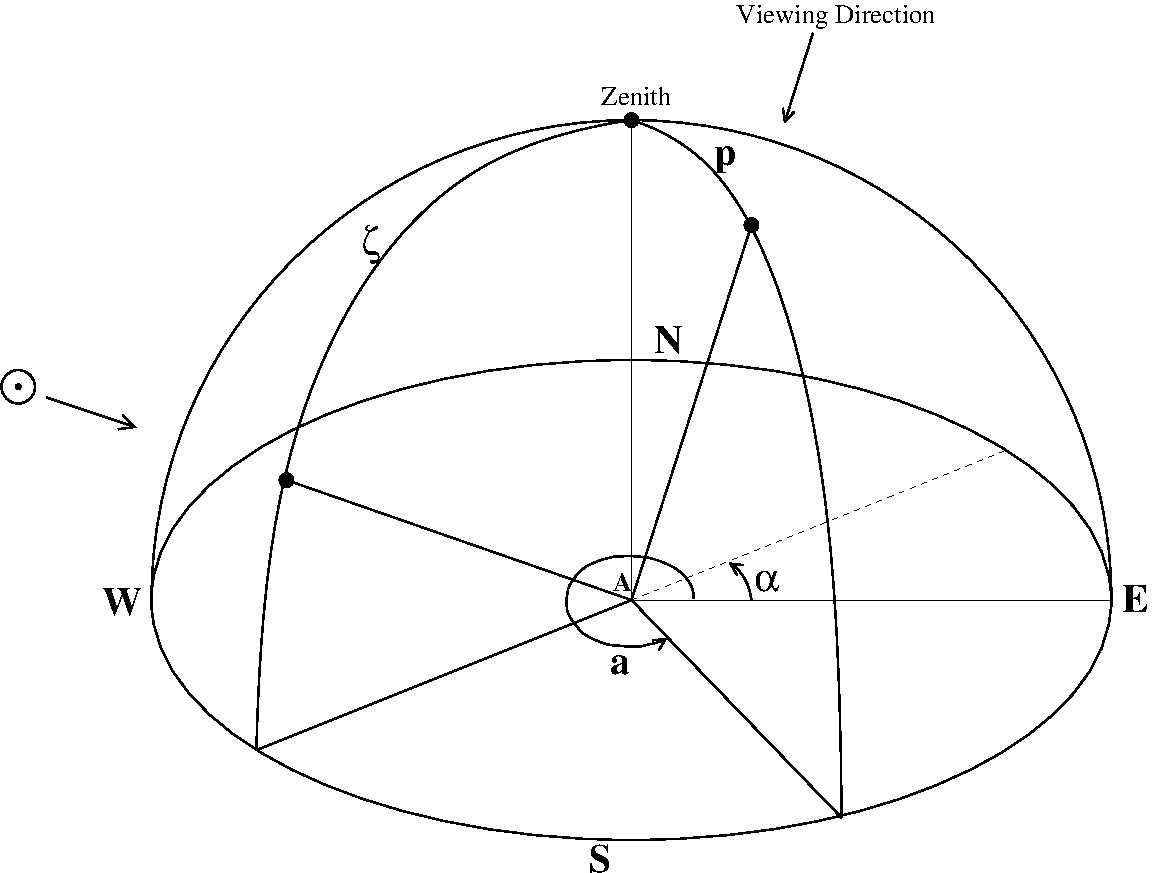
\includegraphics[width=14cm]{view.pdf}}
\html{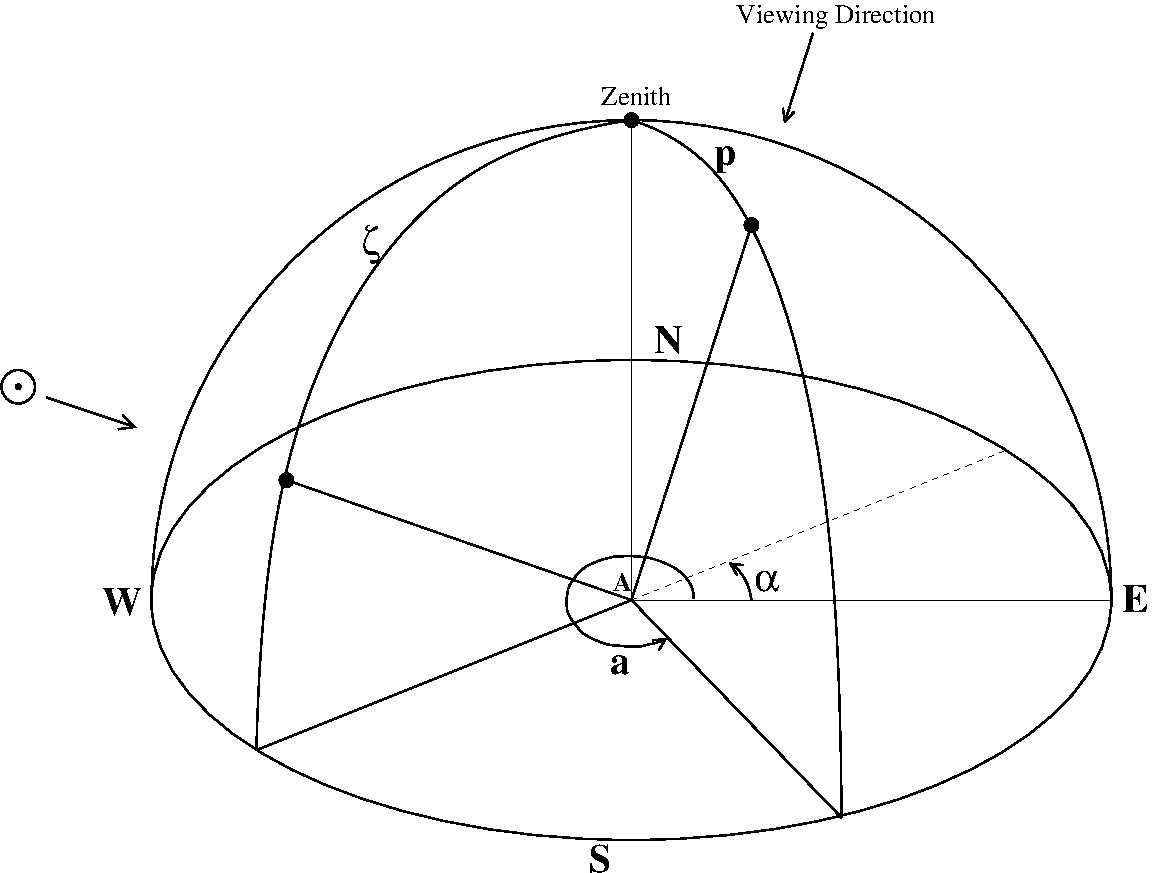
\includegraphics{view.gif}}
\caption{\label{fig:view} Specification of azimuthal and polar viewing angles for the output of radiances.
}
\end{center}
\end{figure}

For each viewing level, the viewing angles are specified in terms of an 
azimuthal and polar viewing angle. These are described most clearly with the 
aid of a diagram. Figure \ref{fig:view} displays the relevant angles from the perspective of point A on the surface. The sun (represented with a dotted circle) is in the south-west, with a solar zenith angle of $\zeta$. The solar azimuth angle represents the forward propogation direction of the solar beam, in this case angle $\alpha$. This has been defined in relation to a zero direction of due east (although the choice of zero direction is arbitrary). The viewing azimuth angle, {\it a} (azim in the {\tt .view} file), must be specified in relation to the same zero direction, anti-clockwise in the same manor as the solar azimuth angle. The viewing polar angle, {\it p} (pol in the {\tt .view} file), is specified in relation to the local zenith. A polar angle of 0 degrees indicates photons travelling straight up and would be applicable for a satellite passing directly overhead. A polar angle of 180 degrees indicates photons travelling straight down and would be applicable for an observer on the surface looking up.

An example {\tt .view} file can be seen in {\tt examples/rc3/rc3.view}.

\section{Using prescribed optical properties}

In the case of clouds and aerosols it is possible to use prescribed optical
properties on given levels. The setting up of a file containing such data is 
described in the previous chapter, but now it is time to discuss its application 
in the program. 

Starting with aerosols, the
option required is {\bf -a} and if this is specified alone the program will
expect to find files of mass mixing ratios on the usual grid (such as
{\tt .soot} for soot): parametrized data from the spectral file will be used.
If {\bf +A} is specified as well the program will first check for the
existence of files with suffixes consisting of the string {\tt op\_} followed
by that for the aerosol (such as {\tt .op\_soot}) which will be assumed to
contain the optical properties of the particular aerosol and these data will
be used instead of a parametrization. Prescribed profiles may be set for
only a selection of the aerosols in the spectral file. Within the program
optical properties will be required on the standard grid, but the levels
in the {\tt .op\_...} file do not have to match this. Using cubic splines,
the program will interpolate from the levels in the file of prescribed
properties to the midpoints of the layers, and will assume that the optical
properties are zero outside the specified range. An example may help. Suppose
that our grid consists of layers with mid-points every 50 mb moving up from
a surface pressure of 1000 mb. Perhaps we have a layer of soot aerosol between
620 and 830 mb, which we specify with optical properties at 630, 680, 730,
790 and 820 mb. In layers with mid-points at 600 mb and lower pressures, or
with mid-points at 850 mb and high pressures, it will be assumed that the
optical properties are zero. The values at 650--800 mb are calculated by
interpolation. There is a potential danger that interpolation may not
conserve the overall optical depth of the layer if the prescribed data are
coarsely resolved or inappropriately chosen: this must be borne in mind
when setting the data. 

The treatment of clouds is similar. To include
clouds we need {\bf -C} as mentioned above. When using prescribed optical
properties there is no need to include splits between convective and layer
cloud in the same grid-box, so we choose the simplest representation, {\bf
-K 1}. The program now expects to be given data for one type of water
droplets and/or one type of ice crystals. To include droplets we use the
option {\bf -d} followed by the type number and to include ice crystals
we use the option {\bf -i} followed by the type number. To use prescribed
profiles of optical properties these type numbers should be set to 0 or
a negative number. The program will then expect files with the suffix
{\tt .op\_water} or {\tt .op\_ice} containing the prescribed optical properties,
which will be interpolated as in the case of aerosols.

\section{Output files}

Output is given in netCDF/CDL files with the following suffixes:
.uflx (upward flux), .dflx (diffuse downward flux), .sflx (direct downward flux),
.vflx (total downward flux: dflx+sflx), .nflx (net downward flux: vflx-uflx),
.hrts (heating rates, K/day), .radn (radiance), .photol (rate of photolysis).


\chapter{Example Calculations}
A collection of example scripts are available in the directory {\tt \$RAD\_DIR/examples}. These cover a variety of usage cases including:

\begin{description}
\item[{\tt rc3}]
: The files in this directory contain the inputs for running the
radiance code on monochromatic data (executable run\_mono) to repeat the
3rd test of the international radiation commission (see Benassi et al.).
These replicate a standard test of monochromatic solar
radiances in specific directions.

\item[{\tt aer\_cmp}]
: An example of using the code to run ICRCCM case 27 (LW) on AER profiles.
The files laer27... contain atmospheric profiles for ICRCCM case27
as used by the AER LBL code given in CDL format. The calculation of
fluxes can be performed using the script run27, which gives an example of
how the code is run. The files aer\_... are the results from the AER LbL code
itself.

\item[{\tt prsc}]
: An example of using prescribed optical
properties for a water cloud. The file {\tt input\_prsc} defines a simple
atmosphere and the script {\tt p1.scr} will run appropriate programs.

\item[{\tt netcdf}]
: Contains data to test the netCDF code ({\tt l\_run\_cdf}). The directory
{\tt netcdf/7460\_28} contains example netCDF input and output 
files for a 1x20 column section of Cloud Resolving Model data. The
directory {\tt netcdf/CIRC\_case6} contains input files for a case study
from the CIRC (Continual Intercomparison of Radiation Codes) project. 
{\tt README} files give instructions for testing.

\item[{\tt aerosols}]
: Contains a script to generate monochromatic single scattering properties
of the aerosols used operationally with HadGEM3.

\item[{\tt droplets}]
: Contains a script to generate cloud droplet optical properties using the
method employed for the operational spectral files.

\item[{\tt corr\_k}]
: Creates a skeleton 300 band LW spectral file, calculates example
water vapour k-terms for bands 38-40 using a cut-down HITRAN line
list, and adds foreign and self broadened continuum coefficients.
CFC-113 coefficients are also added as an example of the use of
cross-section data.

\item[{\tt prep\_data}]
: Test script for scatter\_90, scatter\_average\_90 and prep\_spec provided by
Marc Stringer and Jolene Cook at Reading.

\item[{\tt raw\_input}]
: Demonstrates the use of the raw\_input program to convert column data into
input files (CDL) for the ES code, including the conversion from units of
parts-per-million by volume to kg/kg.

\item[{\tt sp\_lw\_jm}]
: Scripts to create the entire 300 and 9 band LW spectral files from scratch
as intended for the next version of the Met Office global model (GA7).
These take a long time to run (days) and use a lot of space ($\sim$20G).

\item[{\tt sp\_sw\_jm}]
: Scripts to create the entire 260 and 6 band SW spectral files from scratch
as intended for the next version of the Met Office global model (GA7).
These take a long time to run (days) and use a lot of space ($\sim$20G).

\item[{\tt spectral\_var}]
: Adds a look-up table of solar spectral variability data to the GA7
shortwave spectral file. See section~\ref{sec_spectral_var} for further details.

\end{description}

\section{Calculation of spectral radiances}
The following UNIX script is an example of setting up a run to generate spectral
radiances. The names of the spectral files are fictitious, but it should be
possible to run the script with few changes, provided that two 300-band IR
spectral files are provided (or for testing perhaps just two copies of the
standard one). Note, this is an original example script from John Edwards
and uses a number of utilities that while still available in the package
are not otherwise documented here. (Manipulation of input netCDF files can
now generally be done using python or IDL routines.)

There are three main steps. In the first, the standard McClatchey profiles
are copied to a working directory. These profiles do not completely define
the atmospheric state as they omit information on well-mixed gases, so the
missing information is generated. In the second step, because this example
involves the calculation of radiances, the viewing geometry has to be 
specified. A special program generates the input files. The final step 
involves running the radiation code for each band using both files and
writing a line to the output file containing the number of the band and the
radiances calculated form each of the spectral files: this can subsequently
be used as input to a graphics program.

{\small
\begin{verbatim}
#! /bin/ksh
#
# Script to calculate downward surface radiances across the window.
#
SPECTRUM_1=$RAD_DATA/spectra/sp_lw_300_1
SPECTRUM_2=$RAD_DATA/spectra/sp_lw_300_2
#
OUTPUT=zwin
if [ -f $OUTPUT ] ; then rm $OUTPUT ; fi
#
ATM=tro
BASE=lwwin
#
# ------------------------------------------------------
# 1. Make the atmospheric profiles
# ------------------------------------------------------
#
# Copy the raw McClatchey profiles to working files
#
cp  $RAD_DATA/mcc_profiles/one_km/$ATM.tstar $BASE.tstar
#
# The raw McClatchey profile of temperaure is used to define the
# edges of atmospheric layers (suffix .tl).
#
cp  $RAD_DATA/mcc_profiles/one_km/$ATM.t $BASE.tl
#
# Other atmospheric quantities are defined at the mid-points of
# layers, so we make the appropriate mid-points.
#
Cmid_point -o $BASE.mid $BASE.tl
#
# We have now defined the grid. We next make an explicit null
# field to be used in constructing other fields.
#
Cscale_field -R 0.0,1.2e5:0.0 -o $BASE.null -n "nul" -u "None" \
  -L "Null Field" $BASE.mid
#
# Interpolate the temperatures at the mid-points of layers
# (suffix .t) from the edge temperatures. The best option
# for interpolation appears to be linear interpolation of the
# temperature with the logarithm of the pressure (option -lgn).
#
Cinterp -g $BASE.null -o $BASE.t -n "t" -u "K" -L "Central Temperatures" \
  -lgn $BASE.tl
#
# Interpolate the specific humidity to these levels. For ozone and
# water vapour interpolation of the log of the specific humidity in
# the log of the pressure (option -lgg) seems to perform best.
#
Cinterp -g $BASE.null -o $BASE.q -n "q" -u "None" -L "Specific humidity" \
   -lgg $RAD_DATA/mcc_profiles/one_km/$ATM.q
#
# Repeat for ozone.
#
Cinterp -g $BASE.null -o $BASE.o3 -n "o3" -u "None" -L "Ozone mmr" \
   -lgg $RAD_DATA/mcc_profiles/one_km/$ATM.o3
#
# A file is required for each gas in the spectral file.
#
Cinc_field -R 0.0,1.2e5:5.241e-4 -o $BASE.co2 -n "co2" -u "None" \
   -L "CO2 mmr" $BASE.null
Cinc_field -R 0.0,1.2e5:0.2314 -o $BASE.o2 -n "o2" -u "None" \
   -L "O2 mmr" $BASE.null
Cinc_field -R 0.0,1.2e5:0.0 -o $BASE.ch4 -n "ch4" -u "None" \
   -L "CH4 mmr" $BASE.null
Cinc_field -R 0.0,1.2e5:0.0 -o $BASE.n2o -n "n2o" -u "None" \
   -L "N2O mmr" $BASE.null
Cinc_field -R 0.0,1.2e5:0.0 -o $BASE.cfc11 -n "cfc11" -u "None" \
   -L "CFC11 mmr" $BASE.null
Cinc_field -R 0.0,1.2e5:0.0 -o $BASE.cfc12 -n "cfc12" -u "None" \
   -L "CFC12 mmr" $BASE.null
#
# A field of surface albedos is required. In the LW these will
# normally be 0.
#
Cgen_surf_cdl -o $BASE.surf -n alb -L "Surface Albedo" -u "None" \
   -b 0.00 -N 0.0 -T 0.0
#
# ---------------------------------------------------------------
# 2. Generate the viewing geometry.
# ---------------------------------------------------------------
#
# The downward direction is 180.0 degrees in our convention: in the
# IR the azimuth is irrelevant. The atmosphere used here has 32
# layers, so setting a viewing level of 32.0 corresponds to the
# bottom of the 32nd layer.
#
Cgen_view_cdl -o $BASE.view -p 180.0 -a 0.0 -v 32.0 -N 0.0 -T 0.0
#
# ---------------------------------------------------------------
# 3. Run the radiation code.
# ---------------------------------------------------------------
#
# Here we run the radiation code over bands 80 to 120 in the
# the spectral file and evaluate the surface radiance.
#
BAND=80
while [ BAND -le 120 ]
do
#
  Cl_run_cdl -s $SPECTRUM_1 -R $BAND $BAND \
    -B $BASE -C 5 -G 5 0 \
    -g 1 1 -c +R -I +S 3 3 0 0 -T -x zrr
#
# Evaluate the downward radiance at the surface
# The program fval does not work with radiances
# so we use a cheap and nasty approach.
#
  RAD1=$(grep "radiance =" $BASE.radn \
      | awk '{print $3}' | sed -e 's/;//')
#
# Remove the results files from the calculation to
# run with the new spectrum.
#
  resrm $BASE
#
# Repeat for the second spectrum.
  Cl_run_cdl -s $SPECTRUM_2 -R $BAND $BAND \
    -B $BASE -C 5 -G 5 0 \
    -g 1 1 -c +R -I +S 3 3 0 0 -T
#
# Evaluate the downward radiance at the surface.
#
  RAD2=$(grep "radiance =" $BASE.radn \
      | awk '{print $3}' | sed -e 's/;//')
#
# Remove the results files from the calculation to
# run with the new spectrum.
#
  resrm $BASE
#
# Write out the results from the calculations.
  echo $BAND $RAD1 $RAD2 >> $OUTPUT
#
# Move to the next band
  (( BAND = BAND + 1 ))
#
done
\end{verbatim}
}

This example is similar to the IR one in many ways but
we are concerned with calculating SW fluxes.

{\small
\begin{verbatim}
#! /bin/ksh
#
# Script to downward solar fluxes at the surface.
#
SPECTRUM_1=$RAD_DATA/spectra/sp_b220
SPECTRUM_2=$RAD_DATA/spectra/sp_b220_new
#
OUTPUT=zswlst
if [ -f $OUTPUT ] ; then rm $OUTPUT ; fi
#
ATM=tro
BASE=swtest
#
# ------------------------------------------------------
# 1. Make the atmospheric profiles
# ------------------------------------------------------
#
# Copy the raw McClatchey profiles to working files
#
cp  $RAD_DATA/mcc_profiles/one_km/$ATM.tstar $BASE.tstar
#
# The raw McClatchey profile of temperaure is used to define the
# edges of atmospheric layers (suffix .tl).
#
cp  $RAD_DATA/mcc_profiles/one_km/$ATM.t $BASE.tl
#
# Other atmospheric quantities are defined at the mid-points of
# layers, so we make the appropriate mid-points.
#
Cmid_point -o $BASE.mid $BASE.tl
#
# We have now defined the grid. We next make an explicit null
# field to be used in constructing other fields.
#
Cscale_field -R 0.0,1.2e5:0.0 -o $BASE.null -n "nul" -u "None" \
  -L "Null Field" $BASE.mid
#
# Interpolate the temperatires at the mid-points of layers
# (suffix .t) from the edge temperatures. The best option
# for interpolation appears to be linear interpolation of the
# temperature with the logarithm of the pressure (option -lgn).
#
Cinterp -g $BASE.null -o $BASE.t -n "t" -u "K" -L "Central Temperatures" \
  -lgn $BASE.tl
#
# Interpolate the specific humidity to these levels. For ozone and
# water vapour interpolation of the log of the specific humidity in
# the log of the pressure (option -lgg) seems to perform best.
#
Cinterp -g $BASE.null -o $BASE.q -n "q" -u "None" -L "Specific humidity" \
   -lgg $RAD_DATA/mcc_profiles/one_km/$ATM.q
#
# Repeat for ozone.
#
Cinterp -g $BASE.null -o $BASE.o3 -n "o3" -u "None" -L "Ozone mmr" \
   -lgg $RAD_DATA/mcc_profiles/one_km/$ATM.o3
#
# A file is required for each gas in the spectral file.
#
Cinc_field -R 0.0,1.2e5:5.241e-4 -o $BASE.co2 -n "co2" -u "None" \
   -L "CO2 mmr" $BASE.null
Cinc_field -R 0.0,1.2e5:0.2314 -o $BASE.o2 -n "o2" -u "None" \
   -L "O2 mmr" $BASE.null
Cinc_field -R 0.0,1.2e5:0.0 -o $BASE.ch4 -n "ch4" -u "None" \
   -L "CH4 mmr" $BASE.null
Cinc_field -R 0.0,1.2e5:0.0 -o $BASE.n2o -n "n2o" -u "None" \
   -L "N2O mmr" $BASE.null
#
# A field of surface albedos is required. Here we set them to 0.06
# as would be appropriate for sea water.
#
Cgen_surf_cdl -o $BASE.surf -n alb -L "Surface Albedo" -u "None" \
   -b 0.06 -N 0.0 -T 0.0
#
# ---------------------------------------------------------------
# 2. Make the solar fields
# ---------------------------------------------------------------
#
# For two-stream calculations a file of zenith angles is required.
# Azimuthal angles are required only for radiance calculations, but
# a file is produced here for completeness. Fields which have no
# vertical structure can be generated using gen_horiz_cdl.
#
Cgen_horiz_cdl -o $BASE.szen -n szen -L "SOLAR ZENITH" -u "None" \
   -F 30.0 -N 0.0 -T 0.0
Cgen_horiz_cdl -o $BASE.sazim -n azi -L "SOLAR AZIMUTH" -u "None" \
   -F 0.0 -N 0.0 -T 0.0
Cgen_horiz_cdl -o $BASE.stoa -n stoa -L "SOLAR IRRADIANCE" -u "Wm-2" \
   -F 1365.0 -N 0.0 -T 0.0
#
# ---------------------------------------------------------------
# 3. Run the radiation code.
# ---------------------------------------------------------------
#
# Here we run the radiation code over bands 100 to 220 in the
# the spectral files and evaluate the total downward flux at the
# surface.
#
BAND=100
while [ BAND -le 220 ]
do
#
  Cl_run_cdl -s $SPECTRUM_1 -R $BAND $BAND \
    -B $BASE -C 5 -G 5 0 \
    -g 1 1 +R -S -t 2 -x zrr -v 13
#
# Evaluate the downward radiance at the surface
# from the first file. Because there is vertical
# information in this file, the program fval will
# work.
#
  FLX1=$(Cfval -lnn -p 1.013e5 $BASE.vflx)
#
# Remove the results files from the calculation to
# run with the new spectrum.
#
  resrm $BASE
#
# Repeat for the second spectrum.
  Cl_run_cdl -s $SPECTRUM_2 -R $BAND $BAND \
    -B $BASE -C 5 -G 5 0 \
    -g 1 1 -c +R -S -t 2  -v 13
#
# Evaluate the downward flux at the surface.
#
  FLX2=$(Cfval -lnn -p 1.013e5 $BASE.vflx)
#
# Remove the results files from the calculation to
# run with the new spectrum.
#
  resrm $BASE
#
# Write out the results from the calculations.
  echo $BAND $FLX1 $FLX2 >> $OUTPUT
#
# Move to the next band
  (( BAND = BAND + 1 ))
#
done
\end{verbatim}
}

The following script is more complicated. The aim is to generate
values of ice cloud albedo in a 2-D array with the directions
representing spectral band and particle size.

{\small
\begin{verbatim}
#! /bin/ksh
#
# Script to generate data for plots of albedo and absorption as 
# functions of the spectral band and De using the ADA-based
# parametrization for ice crystals.
#
# Ice parametrization
SPECTRUM=$RAD_DATA/spectra/sp_sw_hadgem1_1
ICE_TYPE=7
#
# Define the output file
OUTBASE=ada_bnd_dge
#
#
# Make a working directory:
#
if [ -d work_de ] ; then rm -rf work_de ; fi
mkdir work_de
cd work_de
#
# Make the basic files
#
for ATM in tro mlw saw
  do
   BASE=wk_$ATM
#  Copy the existing CDL-files: this is similar to what we did before.
   cp  $RAD_DATA/mcc_profiles/one_km/$ATM.tstar $BASE.tstar
#  Use the McClatchey levels to define the edges of layers
   cp  $RAD_DATA/mcc_profiles/one_km/$ATM.t $BASE.tl
#  Define the mid-points of these layers, making a null field on 
#  these levels.
   Cmid_point -o $BASE.mid $BASE.tl
   Cscale_field -R 0.0,1.2e5:0.0 -o $BASE.null -n "nul" -u "None" \
      -L "Null Field" $BASE.mid
#  Interpolate the central temperatures from the existing file.
   Cinterp -g $BASE.null -o $BASE.t -n "t" -u "K" -L "Central Temperatures" \
      -lgn $BASE.tl
#  Interpolate specific humidity to these levels, using log-log interpolation.
   Cinterp -g $BASE.null -o $BASE.q -n "q" -u "None" -L "Specific humidity" \
      -lgg $RAD_DATA/mcc_profiles/one_km/$ATM.q
#  Repeat for ozone.
   Cinterp -g $BASE.null -o $BASE.o3 -n "o3" -u "None" -L "Ozone mmr" \
      -lgg $RAD_DATA/mcc_profiles/one_km/$ATM.o3
#
#  Set the mixing ratios of other gases
   Cinc_field -R 0.0,1.2e5:5.241e-4 -o $BASE.co2 -n "co2" -u "None" \
      -L "CO2 mmr" $BASE.null
   Cinc_field -R 0.0,1.2e5:0.2314 -o $BASE.o2 -n "o2" -u "None" \
      -L "O2 mmr" $BASE.null
   Cinc_field -R 0.0,1.2e5:0.0 -o $BASE.ch4 -n "ch4" -u "None" \
      -L "CH4 mmr" $BASE.null
   Cinc_field -R 0.0,1.2e5:0.0 -o $BASE.n2o -n "n2o" -u "None" \
      -L "N2O mmr" $BASE.null
#
#  Make the cloud fields. We create a cloud between 100 and 200 hPa
#  in a tropical atmosphere, with a cloud fraction of 1 by incrementing
#  the null field over the range.
#
   if [ "$ATM" = tro ] 
      then P_CLTOP=1.0e4
      P_CLBASE=2.0e4
      Cinc_field -R $P_CLTOP,$P_CLBASE:1.0 -o $BASE.clfr \
         -n "clfr" -u "None" -L "Cloud Fraction" $BASE.null
   elif [ "$ATM" = mlw ] 
      then P_CLTOP=5.0e4
      P_CLBASE=6.0e4
      Cinc_field -R $P_CLTOP,$P_CLBASE:1.0 -o $BASE.clfr \
         -n "clfr" -u "None" -L "Cloud Fraction" $BASE.null
   elif [ "$ATM" = saw ]
      then P_CLTOP=8.0e4
      P_CLBASE=9.0e4
      Cinc_field -R $P_CLTOP,$P_CLBASE:1.0 -o $BASE.clfr \
         -n "clfr" -u "None" -L "Cloud Fraction" $BASE.null
   fi
#
#  Make the solar fields
   Cgen_horiz_cdl -o $BASE.szen -n szen -L "Solar zenith angle" -u "Degrees" \
      -F 53.0 -N 0.0 -T 0.0
   Cgen_horiz_cdl -o $BASE.stoa -n stoa -L "Solar Irradiance" -u "W.m-2" \
      -F 1365.0 -N 0.0 -T 0.0
   Cgen_horiz_cdl -o $BASE.sazim -n sazim -L "Solar azimuthal angle" \
      -u "Degrees" -F 0.0 -N 0.0 -T 0.0
#
# Make the surface fields
  Cgen_surf_cdl -o $BASE.surf -n alb -L "Surface Albedo" -u "None" \
     -b 0.06 -N 0.0 -T 0.0
#
# A fixed ice water mixing ratio now set. This is an in-cloud value.
# It could be set only within the cloud, but it make no difference if
# it is set on levels where the cloud fraction is zero, as it will 
# have no effect there.
  IWC=0.000025
  Cinc_field -R 0.0,1.2e5:$IWC -o $BASE.iwm -n "iwm" -u "kg/kg" \
      -L "Ice Water Content" $BASE.null
#
# Set the range of mean maximum dimension of the large mode and the
# increment in SI units.
  DL_MIN=0.000010
  DL_INCR=0.000500
#
# Prepare the output file this will hold the dimension of the particle
# the spectral band and the fluxes in that band at the top and bottom
# of the cloud.
  OUTPUT=${OUTBASE}_$ATM
  if [ -f $OUTPUT ] ; then rm $OUTPUT ; fi
  echo "DL  Band UpTop DownTop UpBase DownBase" > $OUTPUT
#
# Use 15 values of DL
  NV=14
  DL=$DL_MIN
  II=0
  while [ II -le NV ]
    do
#
#     The size of ice crystals is set in the ".ire" file, regardless
#     of whether it is an effective radius or some other dimension.
#     The choice must be made based on the parametrization to be used.
#
      if [ -f $BASE.ire ] ; then rm $BASE.ire; fi
      Cinc_field -R 0.0,1.2e5:$DL -o $BASE.ire -n "dl" -u "m" \
         -L "Mean maximum dimension" $BASE.null
      BAND=0
      while [ $BAND -lt 6 ]
        do
           (( BAND = BAND + 1 ))
           resrm $BASE
           Cl_run_cdl -s $SPECTRUM -R $BAND $BAND \
             -B $BASE \
             -C 3 -i $ICE_TYPE -G 5 0 \
             -g 2 -K 1 -r +R -S -t 16 -v 13 -x zrr
           echo $DL $BAND \
               $(Cfval -p $P_CLTOP  -lnn $BASE.uflx) \
              $(Cfval -p $P_CLTOP  -lnn $BASE.vflx) \
             $(Cfval -p $P_CLBASE -lnn $BASE.uflx) \
              $(Cfval -p $P_CLBASE -lnn $BASE.vflx) \
                 >> $OUTPUT
        done
#     The particle size is incremented using the basic calculator bc.
      DL=$( echo "($DL+$DL_INCR)" | bc -l )
      (( II = II + 1 ))
      echo $II
    done
  done
\end{verbatim}
}


\appendix

\chapter{Headers and Suffixes for Processing Observational Data}
The list below gives the recognized headers to be used for raw input and the   
corresponding suffixes for CDL/netCDF files (found in {\tt src/modules\_gen/input\_head\_pcf.f90}).

\begin{tabbing}
\small
{\it Column Heading } \hspace{.5in} \= {\it File Suffix} \hspace{.5in}\= {\it Description }\\
PRESS  \> p         \> Pressure field \\ 
HGT    \> hgt       \> Heights above the surface \\  
TEMP   \> t         \> Temperature \\
PSTAR  \> pstar     \> Surface Pressure \\
TSTAR  \> tstar     \> Surface Temperature \\
O3DEN  \> o3d       \> Mass density of Ozone \\
H2ODEN \> qd        \> Mass density of Water Vapour \\
LWC    \> lwc       \> Liquid Water Content \\
LWM    \> lwm       \> Liquid Water Mass Fraction \\
RE     \> re        \> Effective Radius of Water Droplets \\
LWCCV  \> lwccv     \> Convective Liquid Water Content \\
LWMCV  \> lwmcv     \> Convective Liquid Water Mass Fraction \\
RECV   \> recv      \> Effective Radius of Convective Water Droplets \\
IWC    \> iwc       \> Ice Water Content \\
IWM    \> iwm       \> Ice Water Mass Fraction \\
IRE    \> irecv     \> Effective Radius of Ice Crystals \\
IWCCV  \> iwccv     \> Convective Ice Water Content \\
IWMCV  \> iwmcv     \> Convective Ice Water Mass Fraction \\
IRECV  \> irecv     \> Effective Radius of Convective Ice Crystals \\
CLFRAC \> clfr      \> Cloud Fraction \\
CVFRAC \> ccfr      \> Convective Cloud Fraction \\
WCLFRC \> wclfr     \> Water Cloud Fraction \\
ICLFRC \> iclfr     \> Ice Cloud Fraction \\
CWFRAC \> wccfr     \> Convective Water Cloud Fraction \\
CIFRAC \> iccfr     \> Convective Ice Cloud Fraction \\
TDEW   \> tdw       \> Dew-point Temperature \\
SPH    \> q         \> Specific Humidity \\
HMR    \> hmr       \> Humidity Mixing Ratio \\
RH     \> rh        \> Relative Humidity \\
*      \> null      \> Null Field (used to define pressure levels) \\
UFLX   \> uflx      \> Upward Flux \\
DFLX   \> dflx      \> Diffuse Downward Flux \\
VFLX   \> vflx      \> Total Downward Flux (Direct plus Diffuse) \\
SFLX   \> sflx      \> Direct Flux \\
NFLX   \> nflx      \> Net Downward Flux \\
HRTS   \> hrts      \> Heating Rate (Kelvin per day) \\
TAU    \> tau       \> Optical depth \\
SSA    \> ssa       \> Albedo of Single Scattering \\
ASYM   \> gsc       \> Asymmetry of Single Scattering \\
FRWSC  \> fsc       \> Forward scattering parameter \\
PLANCK \> plk       \> Planck function \\
DISCRD \> *         \> Discard Column \\
TLEV   \> tl        \> Temperature on levels \\
SZEN   \> szen      \> Solar zenith angle \\
SAZIM  \> sazim     \> Solar azimuthal angle \\
STOA   \> stoa      \> Solar Irradiance at TOA \\
SURF   \> surf      \> Type of surface \\
POLAR  \> vwpol     \> Polar viewing angle \\
AZIM   \> vwazim    \> Azimuthal viewing angle \\
RADN   \> radn      \> Radiance \\
SRFCHR \> surf      \> Surface characteristics \\
OPWT   \> op\_water \> Optical data for droplets \\
OPICE  \> op\_ice   \> Optical data for ice crystals \\
OPSS   \> ss        \> Single scattering properties \\
ISOS   \> isos      \> Isotropic source \\
GEOM   \> view      \> Viewing Geometry \\
PHOTOL \> photol    \> Rate of photolysis \\
PLEV   \> pl        \> Pressure on Levels \\
\end{tabbing}

An asterisk in a column indicates that there is no corresponding header
or suffix for this field since the corresponding functionality would be
inappropriate.

\section{Gases}

The gases are specified as mass mixing ratios using filenames based on
their chemical symbols, except in the case of water vapour where the latter
{\tt q} is used.

\begin{tabbing}
\small
{\it Column Heading} \hspace{.5in}\= {\it File Suffix} 
\hspace{.5in}\= {\it Name of Gas } \\
H2O     \> q       \> Water Vapour \\
CO2     \> co2     \> Carbon dioxide \\
O3      \> o3      \> Ozone \\ 
N2O     \> n2o     \> Nitrous Oxide \\
CO      \> co      \> Carbon monoxide \\
CH4     \> ch4     \> Methane \\
O2      \> o2      \> Oxygen \\
NO      \> no      \> Nitrogen monoxide \\
SO2     \> so2     \> Sulphur dioxide \\
NO2     \> no2     \> Nitrogen dioxide \\
NH3     \> nh3     \> Ammonia \\
HNO3    \> hno3    \> Nitric acid \\
N2      \> n2      \> Nitrogen \\
CFC11   \> cfc11   \> CFC-11 \\
CFC12   \> cfc12   \> CFC-12 \\
CFC113  \> cfc113  \> CFC-113 \\
HCFC22  \> hcfc22  \> HCFC-22 \\
HFC125  \> hfc125  \> HFC-125  \\
HFC134A \> hfc134a \> HFC-134a \\
CFC114  \> cfc114  \> CFC-114 \\
TiO     \> tio     \> Titanium oxide \\
VO      \> vo      \> Vanadium oxide \\
H2      \> h2      \> H2-H2 CIA \\
He      \> he      \> H2-He CIA \\
OCS     \> ocs     \> Carbonyl sulphide \\
\end{tabbing}

\section{Aerosols}

In the case of aerosols the headings for the columns and the suffixes for 
the files are:

\begin{tabbing}
\small
{\it Column Heading} \hspace{.5in}\= {\it File Suffix} 
\hspace{.5in}\= {\it Name of Aerosol} \\
WTSOL    \> wtsol     \>  Water Soluble Aersol         \\
DUST     \> dust      \>  Dust-like Aerosol            \\
OCN      \> ocn       \>  Oceanic Aerosol              \\
SOOT     \> soot      \>  Sooty Aerosol                \\
ASH      \> ash       \>  Volcanic ash                 \\
SULPH    \> sulph     \>  Sulphuric acid droplets      \\
NH4SO4   \> nh4so4    \>  Ammonium Sulphate            \\
AUNCH    \> aunch     \>  Uncharacterized Aerosol      \\
SAHARA   \> sahara    \>  Saharan Dust Aerosol         \\
ACCUM    \> accum     \>  Accumulation SO4 Aerosol     \\
AITKEN   \> aitken    \>  Aitken-mode SO4 Aerosol      \\
FRSOOT   \> frsoot    \>  Fresh Soot Aerosol           \\
AGSOOT   \> agsoot    \>  Aged Soot Aerosol            \\
NACL     \> nacl      \>  Generic Sodium Chloride      \\
NACLFLM  \> naclflm   \>  Sodium Chloride (Film mode)  \\
NACLJET  \> nacljet   \>  Sodium Chloride (Jet mode)   \\
DUSTDIV1 \> dustdiv1  \>  Dust aerosol (division 1)    \\
DUSTDIV2 \> dustdiv2  \>  Dust aerosol (division 2)    \\
DUSTDIV3 \> dustdiv3  \>  Dust aerosol (division 3)    \\
DUSTDIV4 \> dustdiv4  \>  Dust aerosol (division 4)    \\
DUSTDIV5 \> dustdiv5  \>  Dust aerosol (division 5)    \\
DUSTDIV6 \> dustdiv6  \>  Dust aerosol (division 6)    \\
BIOMS1   \> bioms1    \>  Biomass aerosol (division 1) \\
BIOMS2   \> bioms2    \>  Biomass aerosol (division 2) \\
BIOGENIC \> biogenic  \>  Biogenic aerosol             \\
FROCFF   \> frocff    \>  Fresh fossil-fuel org. carbon\\
AGOCFF   \> agocff    \>  Aged fossil-fuel org. carbon \\
DELTA    \> delta     \>  Unspecified (delta) aerosol  \\
NITRATE  \> nitrate   \>  Ammonium nitrate aerosol     \\
DUST2BIN1\> dust2bin1 \>  Two-bin Dust aerosol (div 1) \\
DUST2BIN2\> dust2bin2 \>  Two-bin Dust aerosol (div 2) \\

\end{tabbing}

File suffixes for the optical properties of each aerosol are as above, beginning with the letters op\_ e.g. .dust becomes .op\_dust.

\section{Units}

The recognized units for use in headers are these:

\begin{tabbing}
\small
{\it Symbol for Unit } \hspace{.5in}
\= {\it Name of Unit } \\
PA    \> Pascal \\
MB    \> Millibar \\ 
K     \> Kelvin \\
M     \> Metre \\
KM    \> Kilometre \\
UM    \> Micron \\
KGM-3 \> Kilograms per cubic metre \\
GM-3  \> Grams per cubic metre \\
KGM-2 \> Kilograms per square metre \\
GM-2  \> Grams per square metre \\
GKG-1 \> Grams per kilogram \\
GG-1  \> Grams per gram \\
NONE  \> Dimensionless quantity \\
M-3   \> Number per cubic metre \\
CM-3  \> Number per cubic centimetre \\
WM-2  \> Watts per square metre \\
C     \> Degrees Celsius \\
PPMV  \> Parts per million by volume \\
\end{tabbing}


\end{document}
